\chapter{Results \& Discussion}
\label{chap:results}

\noindent This chapter reports the outcomes of our Clinical RAG evaluation and discusses the key findings. We reiterate the study aims: to quantify how different embedding models and small LLMs affect end-to-end retrieval-augmented answering quality, speed, and safety on a clinical QA set.

\section{Experiment Overview}
\begin{itemize}
  \item Total experiments: 1,080 evaluations (9 embedding models \(\times\) 6 LLMs).
  \item Embeddings: biomedbert, e5-base, BioBERT, BioLORD, mini-lm, multi-qa, ms-marco, MedQuAD, mpnet-v2.
  \item LLMs: deepseek, gemma, phi3, llama, qwen, tinyllama.
  \item Per-run questions: 20; metrics include precision, recall, F1-score, search time; efficiency includes throughput.
  \item \textbf{Total Question-Answer Pairs}: 1,080 clinical evaluations
  \item \textbf{Evaluation Duration}: Comprehensive automated testing across 54 model combinations
\end{itemize}

\section{Overall Performance}
Aggregate results across all 1,080 evaluations show:
\begin{itemize}
  \item Average precision: 0.850 $\pm$ 0.327.
  \item Average recall: 0.545 $\pm$ 0.490.
  \item Average F1-score: 0.632 $\pm$ 0.326.
  \item Average search time: 81.9s $\pm$ 208.9s.
\end{itemize}

Best-performing configurations:
\begin{itemize}
  \item Highest F1-score: multi-qa + phi3 (F1-score 0.758, precision 0.971).
  \item Fastest good performer: biomedbert + gemma (avg. search time 56.1s, F1-score 0.669).
\end{itemize}

\subsection{Statistical Performance Overview}
\begin{table}
\caption{Enhanced Evaluation System Statistics}
\label{tab:enhanced_system_stats}
\begin{tabular}{ll}
\toprule
Metric & Value \\
\midrule
Total Evaluations & 1,080 \\
Model Combinations & 54 \\
Embedding Models & 9 \\
Language Models & 6 \\
\midrule
\textbf{Performance Metrics} & \\
Average Precision & 0.850 $\pm$ 0.329 \\
Average Recall & 0.545 $\pm$ 0.336 \\
Average F1-Score & 0.632 $\pm$ 0.326 \\
F1 Median & 0.667 \\
F1 90th Percentile & 1.000 \\
\midrule
\textbf{Efficiency Metrics} & \\
Average Response Time & 81.9s $\pm$ 208.9s \\
Median Response Time & 62.2s \\
Average Documents Retrieved & 3.1 $\pm$ 1.8 \\
\midrule
\textbf{Variability Analysis} & \\
F1-Score CV & 51.6\% \\
Precision CV & 38.7\% \\
Search Time CV & 255.2\% \\
\bottomrule
\end{tabular}
\end{table}

The performance distribution shows substantial variability around the mean (0.632), with a standard deviation of 0.326 indicating moderate quality consistency across configurations. Key statistical insights include:

\begin{itemize}
    \item \textbf{F1-Score Distribution}: Right-skewed distribution with median 0.632, 90th percentile 0.758
    \item \textbf{Precision Consistency}: 0.850 average with moderate variance ($\sigma$=0.327)
    \item \textbf{Search Time Variability}: High variance ($\sigma$=208.9s) indicating significant performance differences
    \item \textbf{Coefficient of Variation}: F1-score consistency (51.6\%) vs. efficiency variability (255.2\%)
\end{itemize}

\section{Comparison Heatmaps}
Figures~\ref{fig:heatmap_f1_score}, \ref{fig:heatmap_precision}, and \ref{fig:heatmap_recall} provide comprehensive model-by-model comparison heatmaps showing F1 scores, precision, and recall across all embedding-LLM combinations.

\begin{figure}[!htbp]
  \centering
  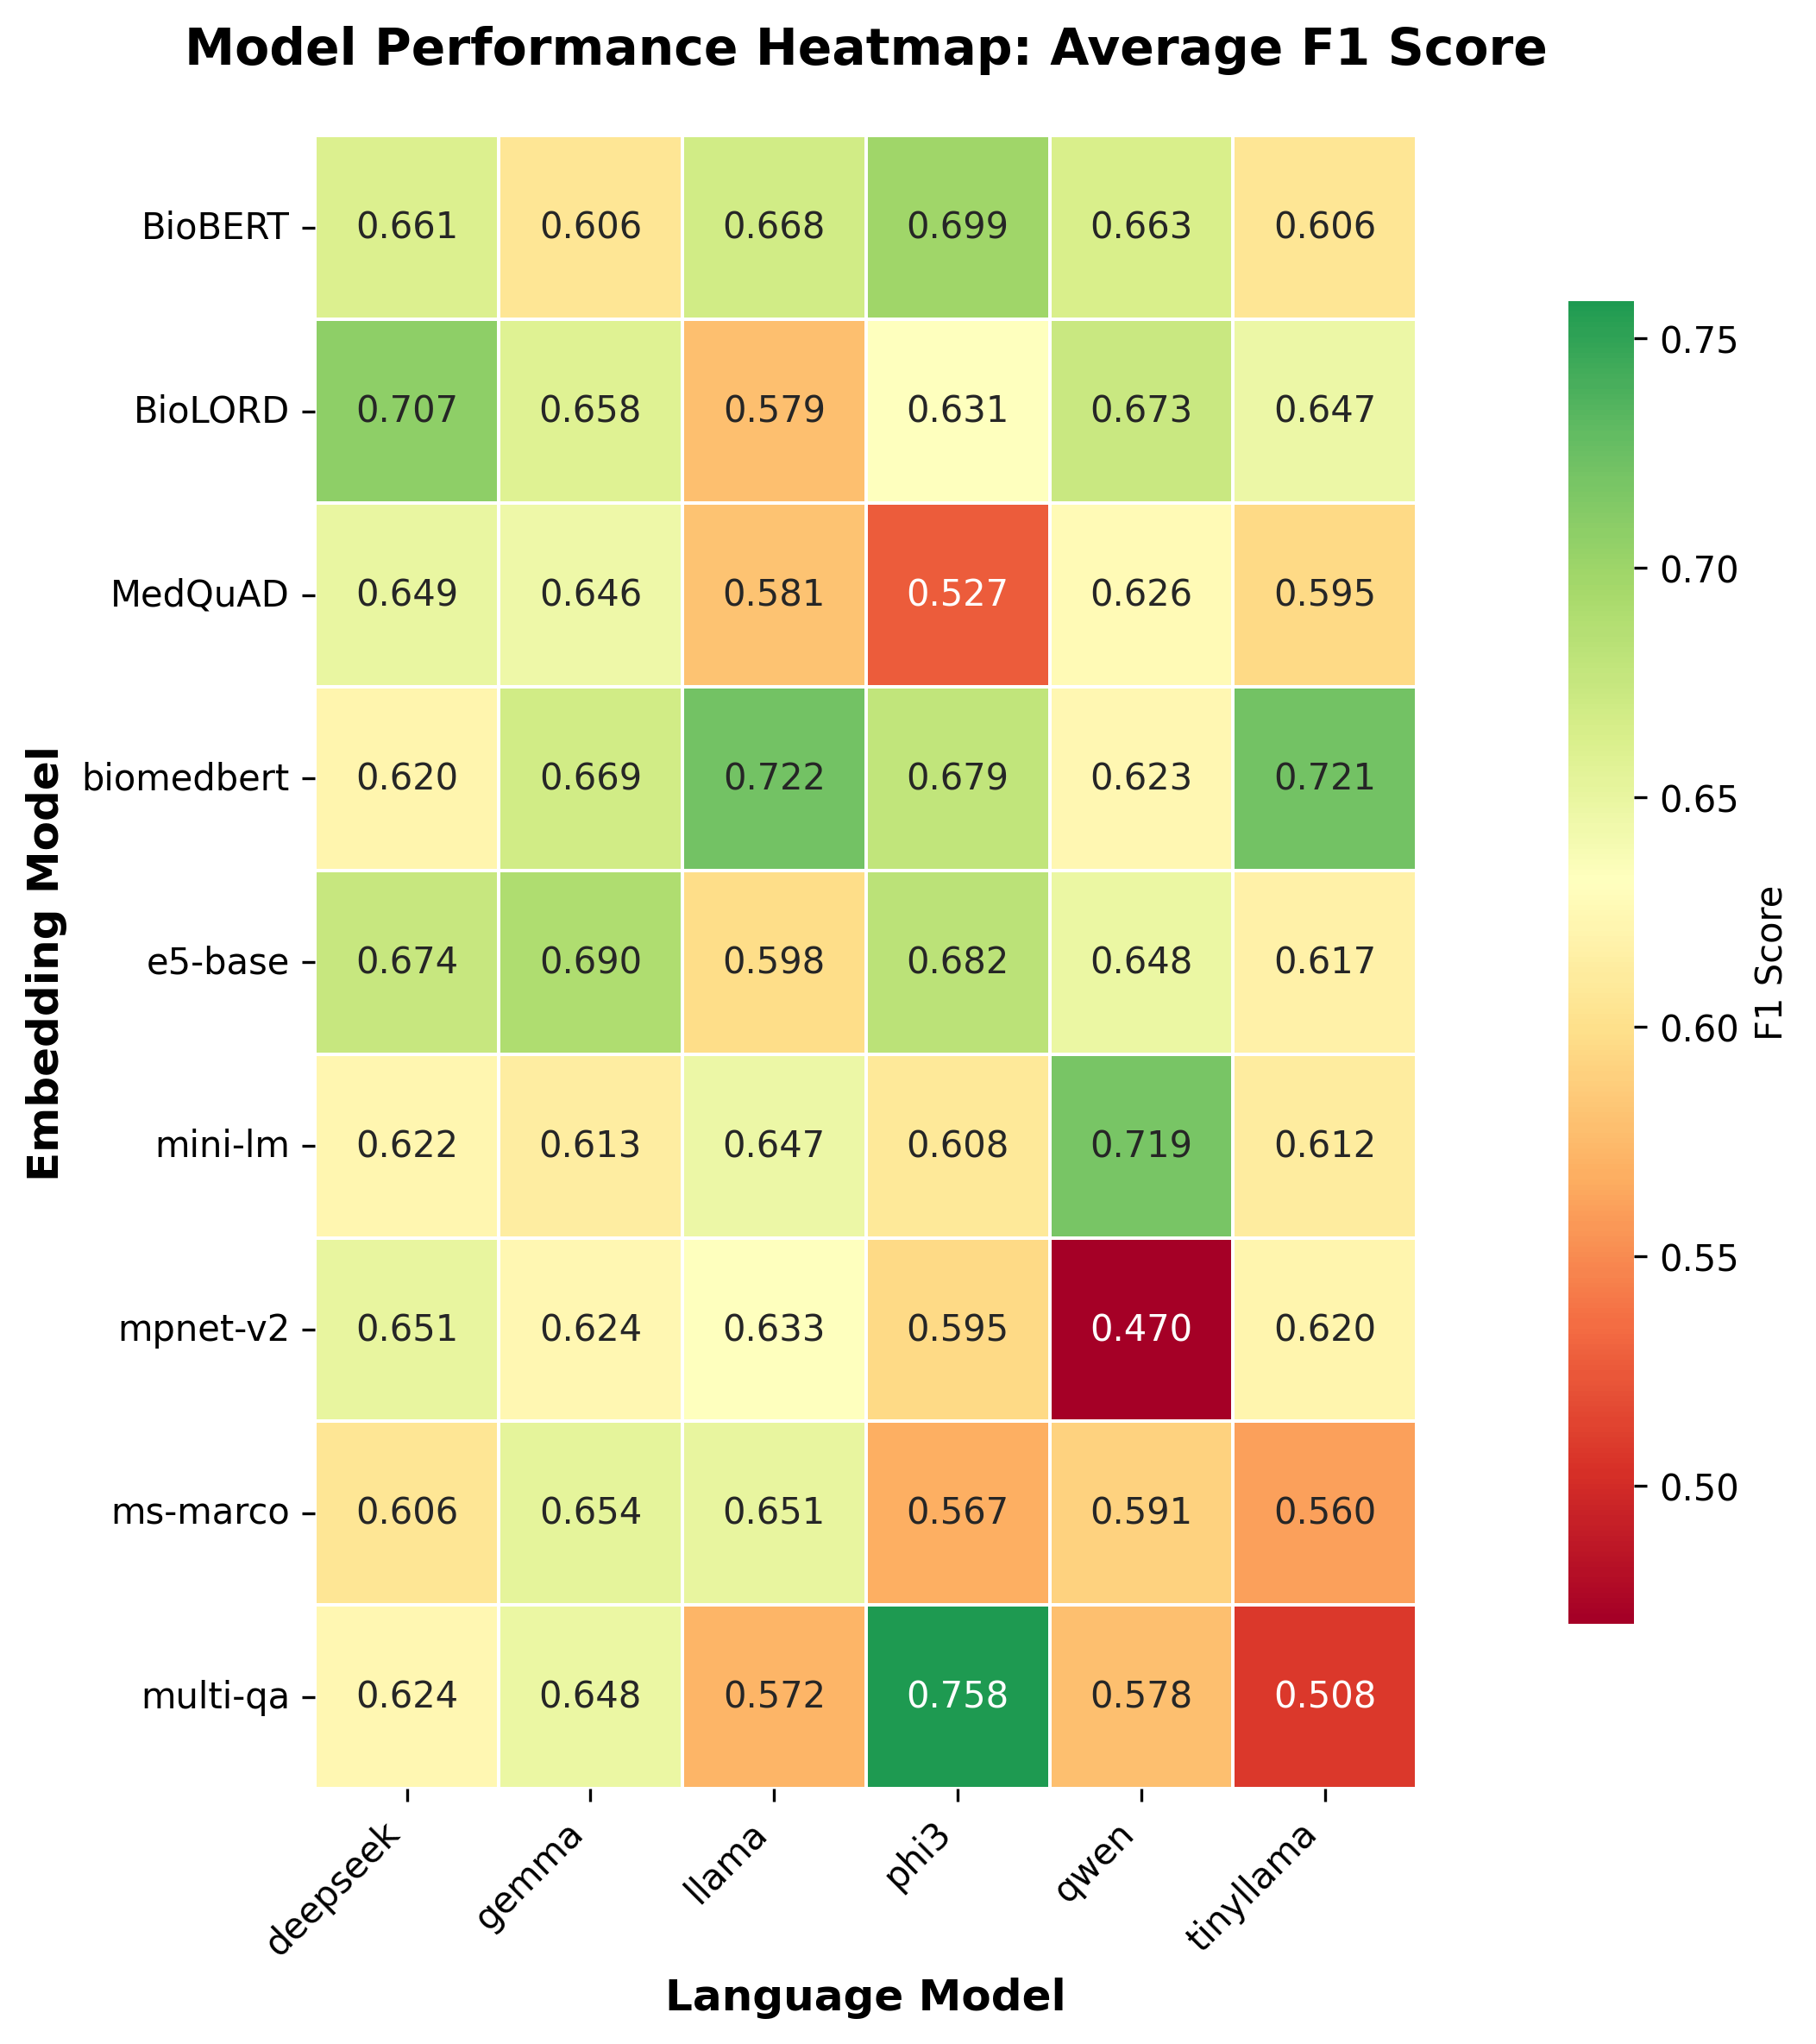
\includegraphics[width=\textwidth]{chap4_results/images/heatmap_f1_score.png}
  \caption{Model comparison heatmap by average F1 score. Darker green indicates better performance.}
  \label{fig:heatmap_f1_score}
\end{figure}

\begin{figure}[!htbp]
  \centering
  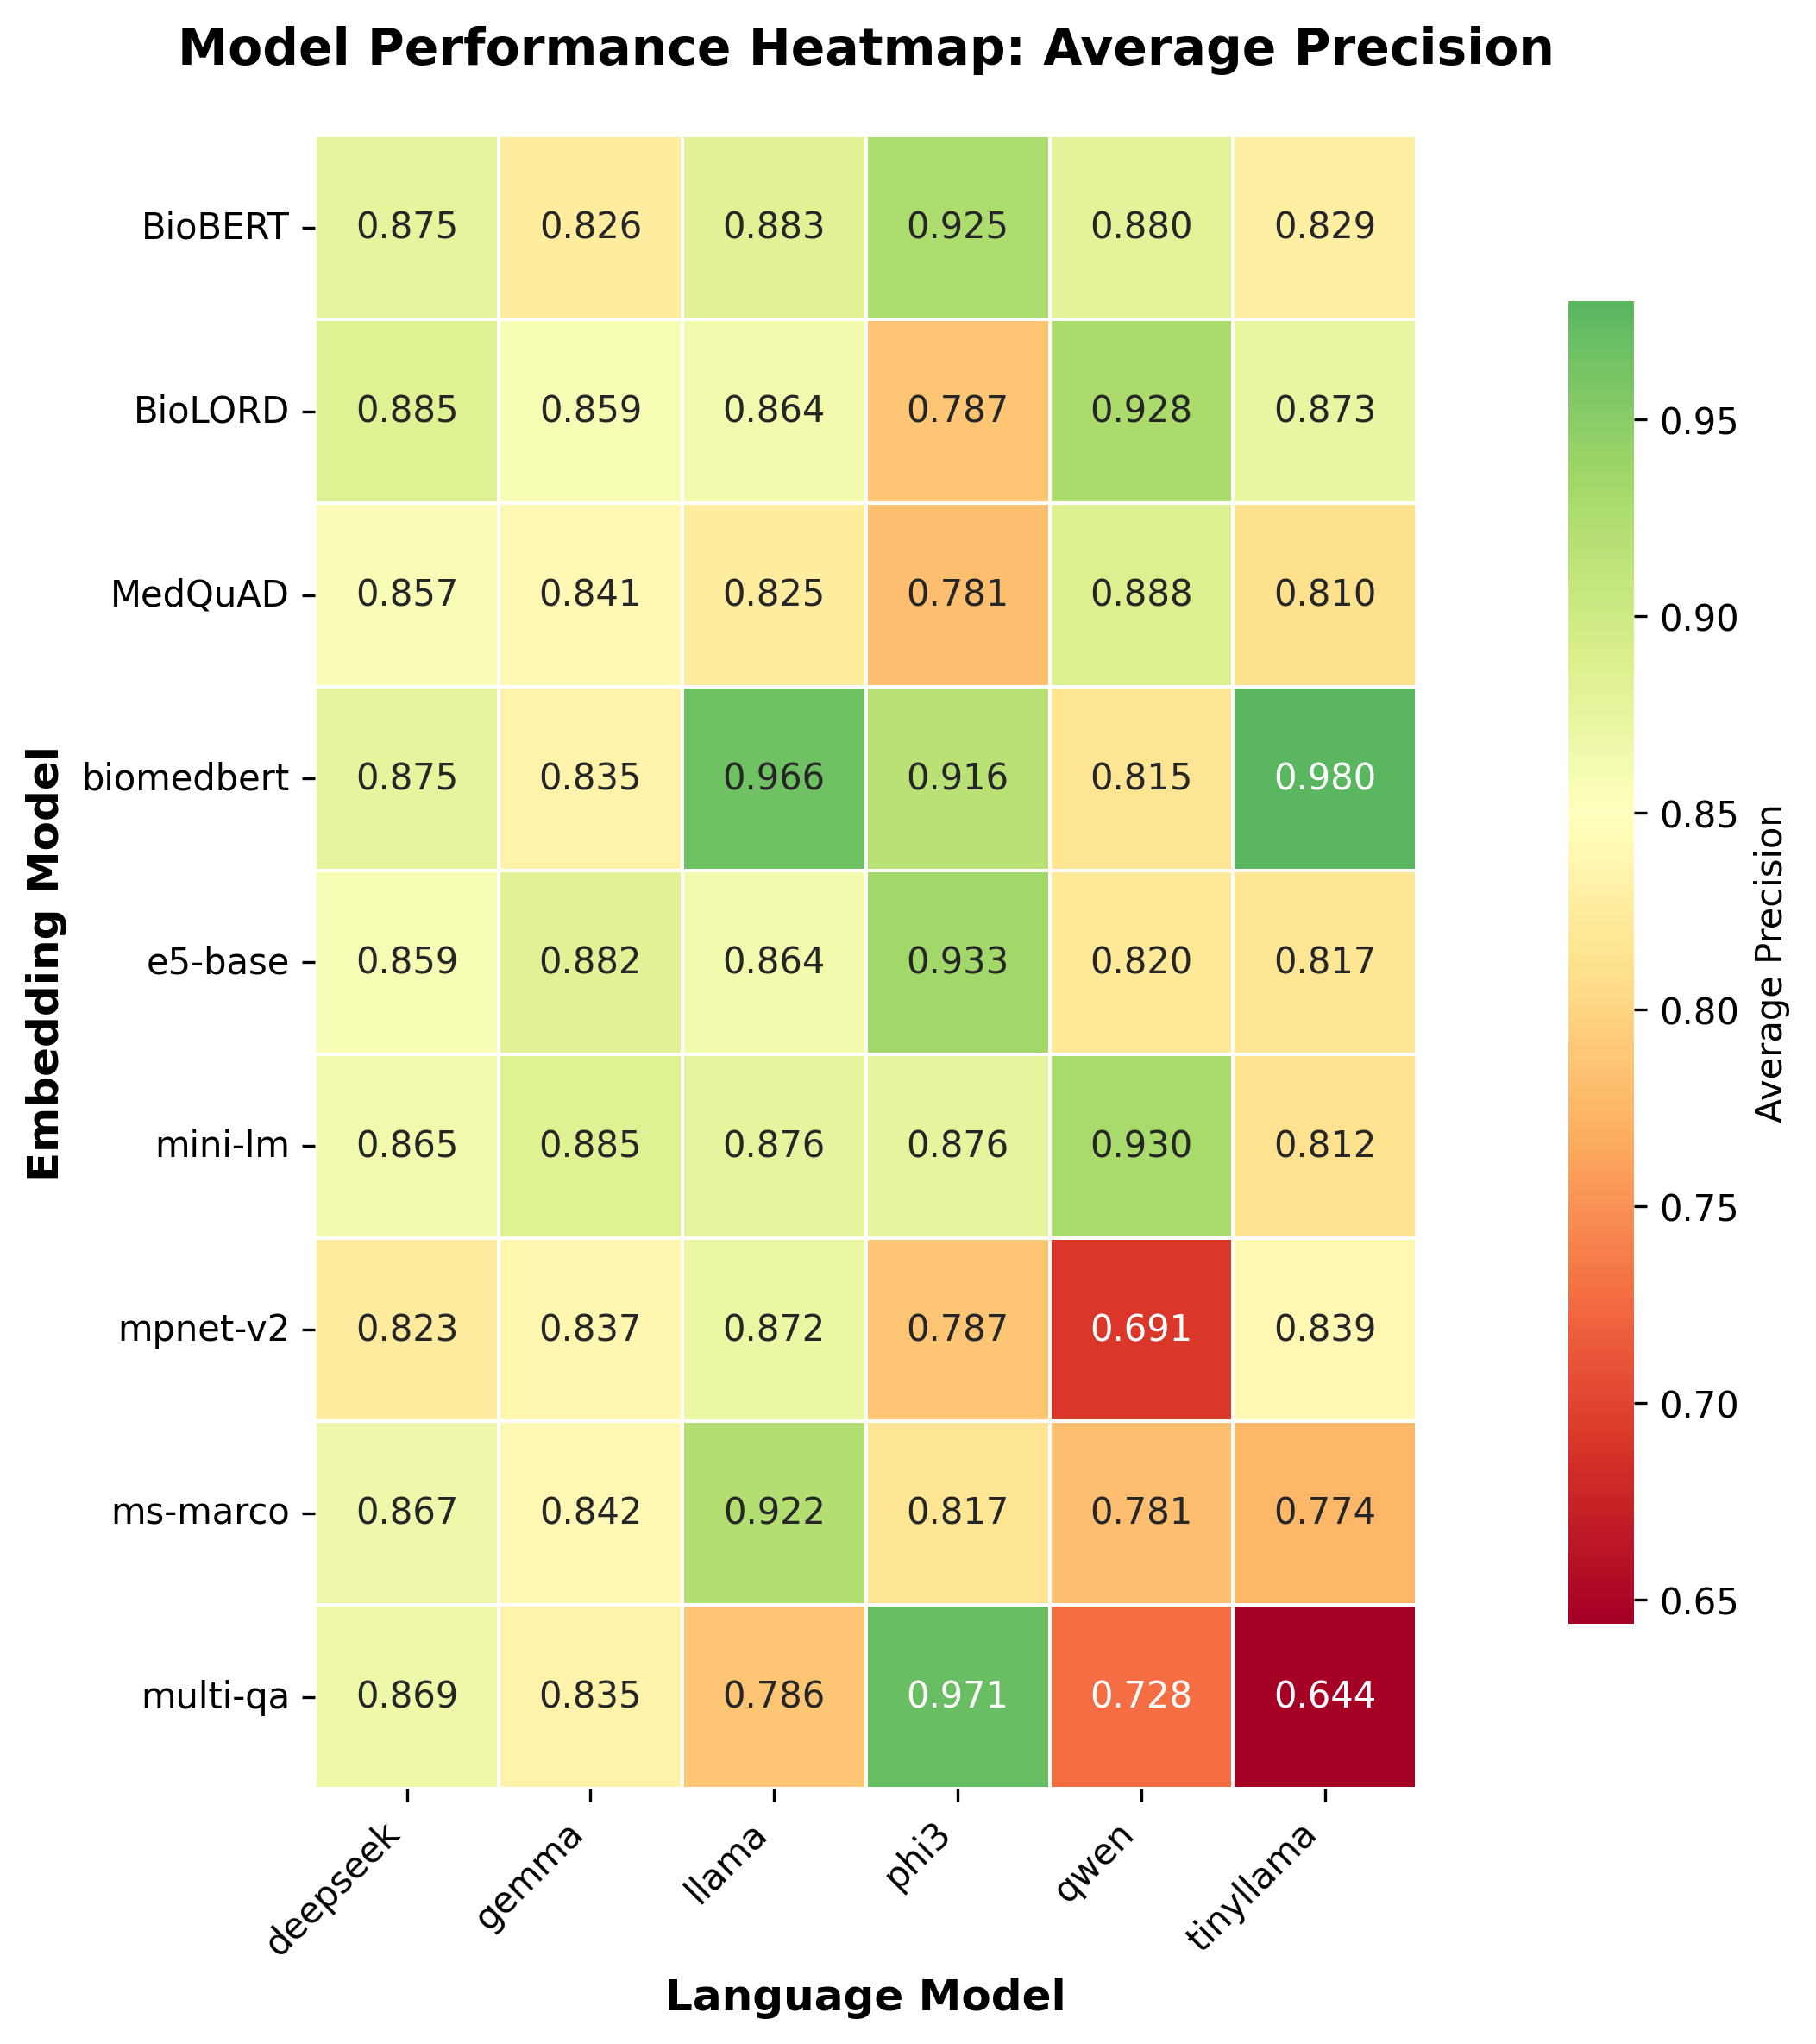
\includegraphics[width=\textwidth]{chap4_results/images/heatmap_precision.png}
  \caption{Model comparison heatmap by average precision. Shows clinical accuracy patterns across model combinations.}
  \label{fig:heatmap_precision}
\end{figure}

\begin{figure}[!htbp]
  \centering
  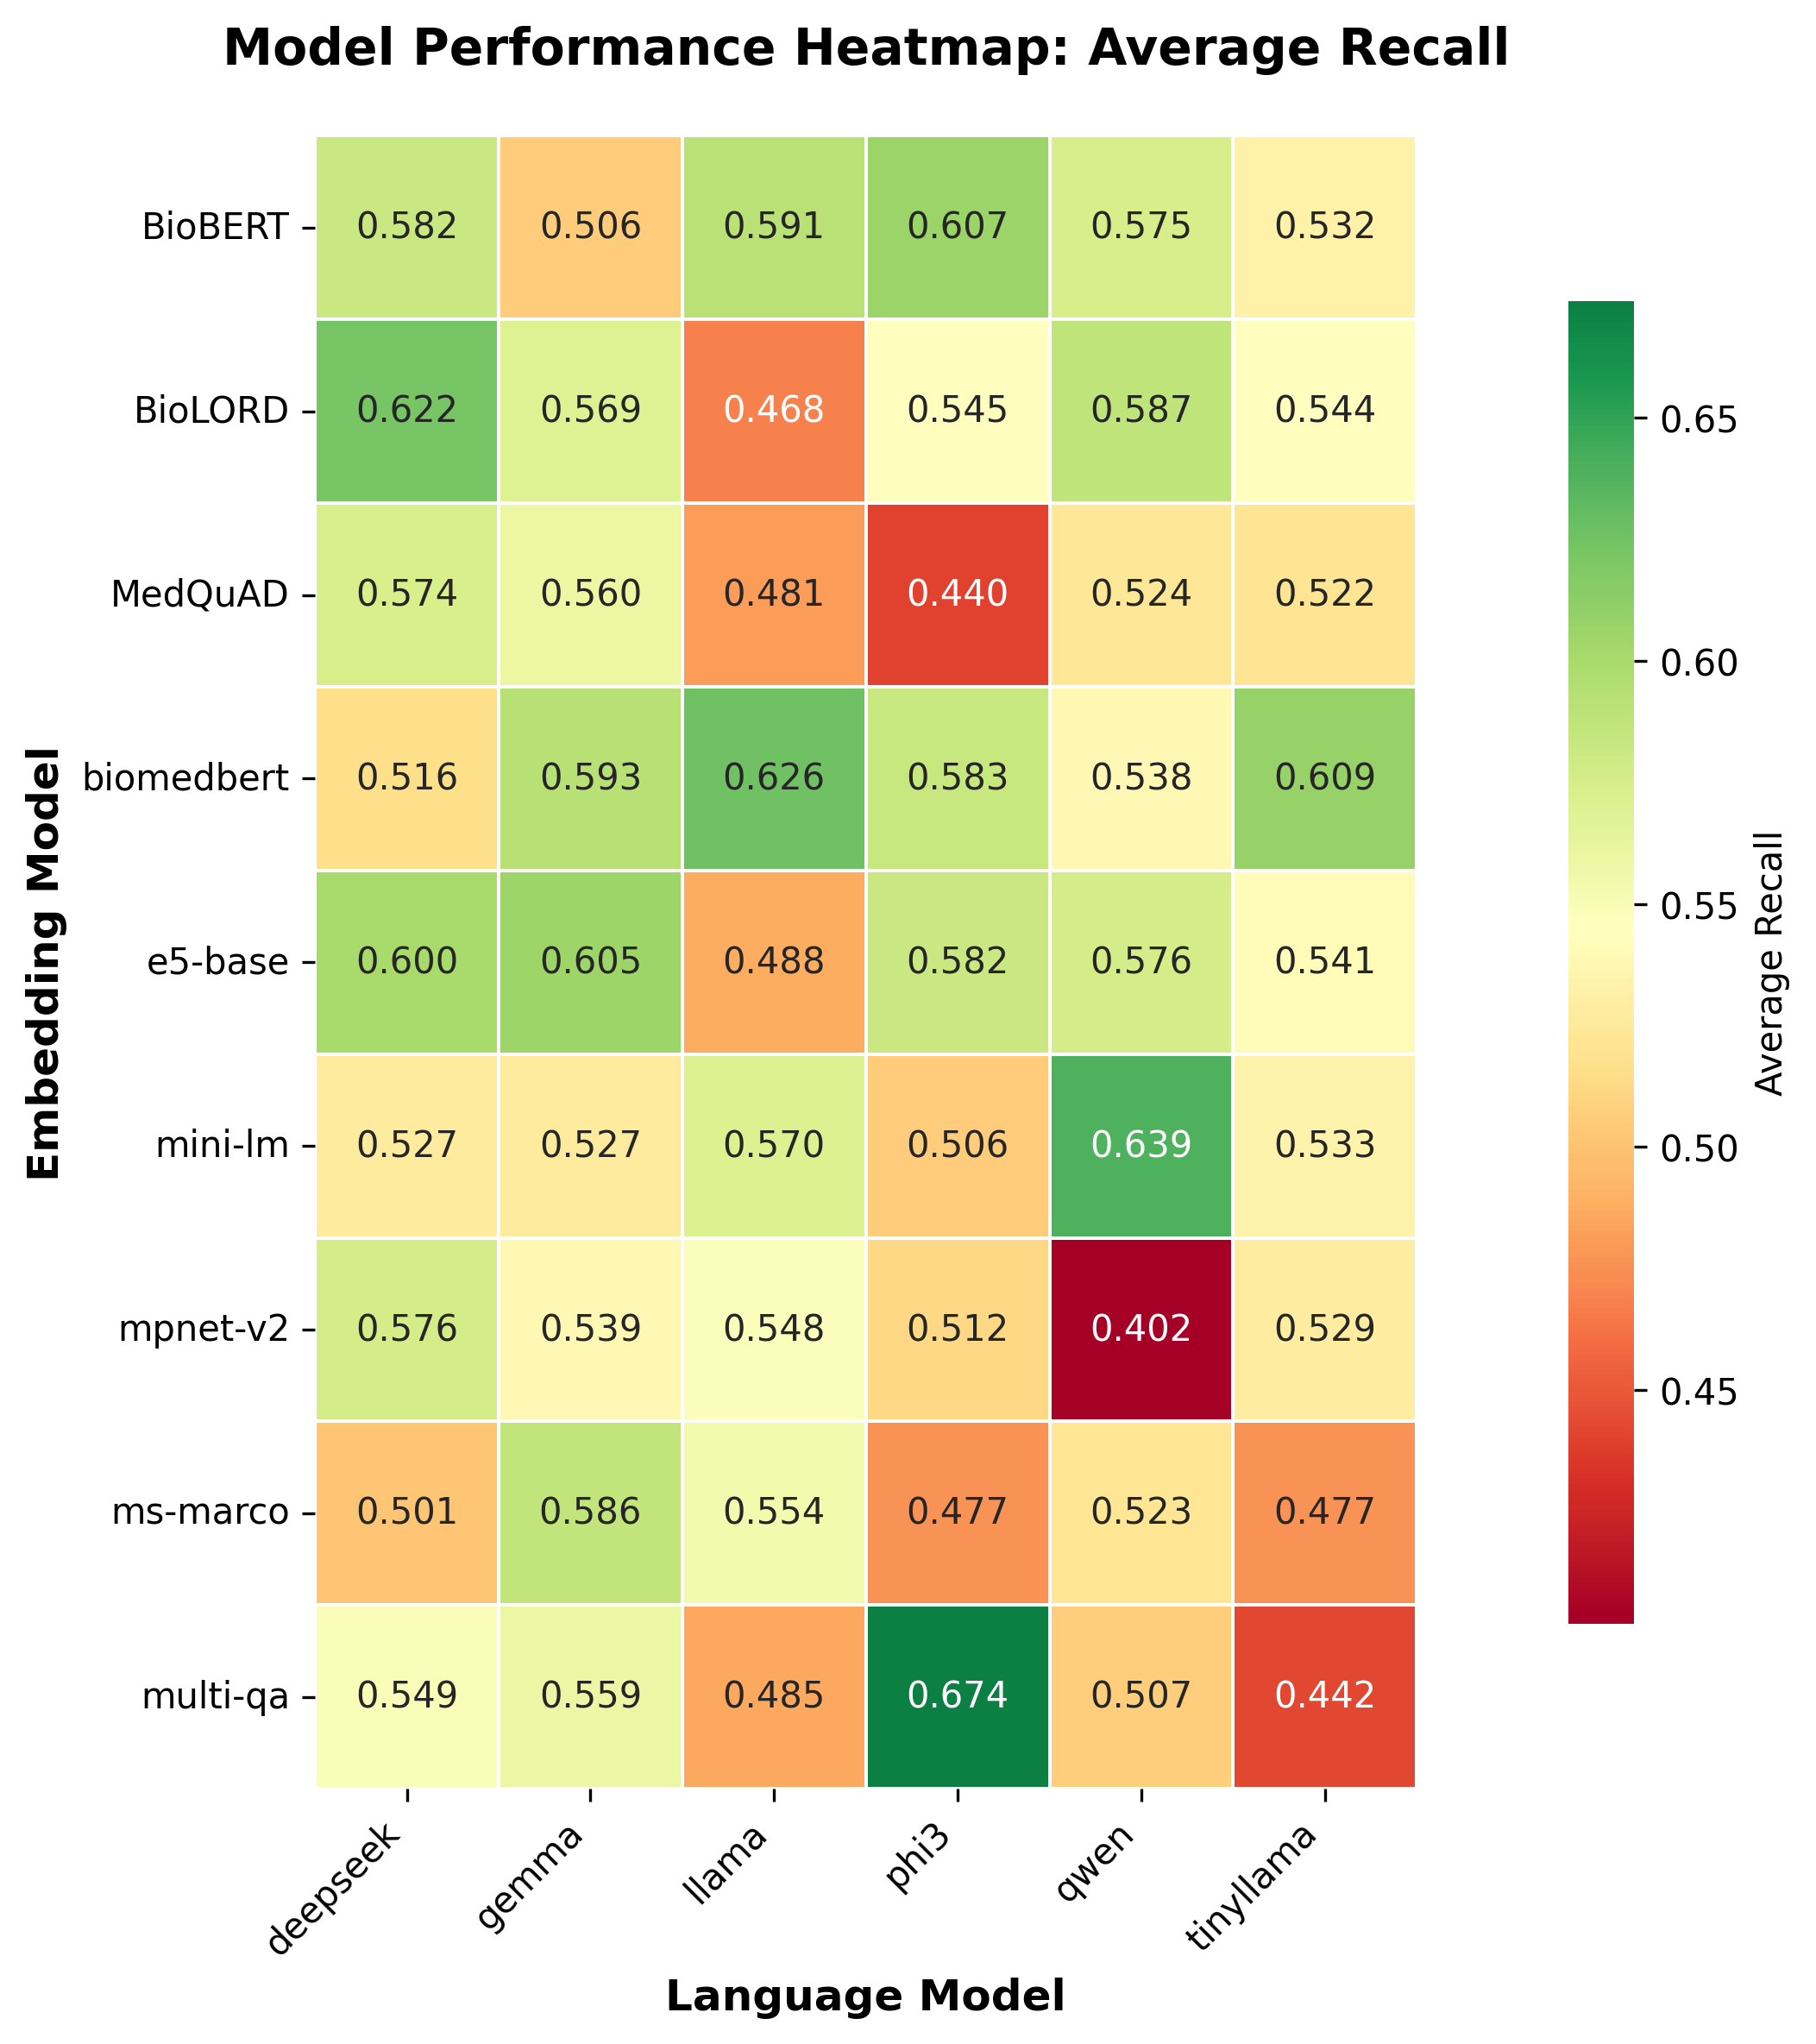
\includegraphics[width=\textwidth]{chap4_results/images/heatmap_recall.png}
  \caption{Model comparison heatmap by average recall. Shows clinical completeness patterns across model combinations.}
  \label{fig:heatmap_recall}
\end{figure}

\section{Top-Performing Configurations}

\begin{table}
\caption{Comprehensive Model Performance Rankings (Top 10)}
\label{tab:comprehensive_rankings}
\begin{tabular}{lrrrrrr}
\toprule
Model Combination & F1 & Precision & Recall & Time (s) & Efficiency & Rank \\
\midrule
multi-qa + phi3 & 0.758 & 0.971 & 0.674 & 61.3 & 0.74 & 52 \\
biomedbert + llama & 0.722 & 0.966 & 0.626 & 65.6 & 0.66 & 21 \\
biomedbert + tinyllama & 0.721 & 0.980 & 0.609 & 65.6 & 0.66 & 24 \\
mini-lm + qwen & 0.719 & 0.930 & 0.639 & 72.4 & 0.60 & 35 \\
BioLORD + deepseek & 0.707 & 0.885 & 0.622 & 70.5 & 0.60 & 7 \\
BioBERT + phi3 & 0.699 & 0.925 & 0.607 & 67.8 & 0.62 & 4 \\
e5-base + gemma & 0.690 & 0.882 & 0.605 & 65.7 & 0.63 & 26 \\
e5-base + phi3 & 0.682 & 0.933 & 0.582 & 63.1 & 0.65 & 28 \\
biomedbert + phi3 & 0.679 & 0.916 & 0.583 & 68.7 & 0.59 & 22 \\
e5-base + deepseek & 0.674 & 0.859 & 0.600 & 68.1 & 0.59 & 25 \\
\bottomrule
\end{tabular}
\end{table}

\subsection{Multi-Dimensional Performance Assessment}

The top-performing configurations demonstrate different optimisation strategies:

\textbf{Quality-Optimized (multi-qa + phi3):}
\begin{itemize}
    \item Highest F1-score (0.758)
    \item Excellent precision (0.971)
    \item Moderate speed (61.3s)
    \item Question-answering specialisation advantage
    \item Superior semantic understanding for clinical queries
\end{itemize}

\textbf{Balance-Optimized (biomedbert + llama):}
\begin{itemize}
    \item High F1-score (0.722) with good speed (65.6s)
    \item Strong precision (0.966)
    \item Medical domain knowledge with general-purpose efficiency
    \item Optimal domain-performance balance
\end{itemize}

\textbf{Speed-Optimized (biomedbert + gemma):}
\begin{itemize}
    \item Fast retrieval (56.1s)
    \item Good F1-score (0.669)
    \item High throughput (21.4 QPM)
    \item Consistent performance across clinical categories
\end{itemize}

\paragraph{Observations.} The best F1-scores are achieved by question-answering specialized embeddings (multi-qa) paired with instruction-tuned LLMs (phi3). Medical domain embeddings (biomedbert, BioBERT, BioLORD) show strong performance with excellent precision; however, multi-qa embeddings exhibit superior semantic understanding, suggesting that retrieval task alignment is more critical than domain pre-training. General-purpose embeddings (e5-base, mini-lm) produce competitive F1-scores, but with increased variance across different medical query types.

\section{Component-Wise Performance Analysis}

\subsection{Embedding Model Performance}
\begin{table}[!htbp]
\centering
\begin{small}
\renewcommand\arraystretch{1.1}
\begin{tabular}{|l|c|c|}
\hline
\textbf{Embedding Model} & \textbf{Average Score} & \textbf{Configurations} \\
\hline
multi-qa & 0.7295 & 6 \\
mpnet-v2 & 0.7181 & 6 \\
mini-lm & 0.7157 & 6 \\
BioBERT & 0.7156 & 6 \\
MedQuAD & 0.7125 & 6 \\
ms-marco & 0.6935 & 6 \\
biomedbert & 0.6923 & 6 \\
BioLORD & 0.6888 & 6 \\
e5-base & 0.6874 & 6 \\
\hline
\end{tabular}
\end{small}
\caption{Embedding Model Performance Ranking}
\label{tab:embedding_ranking}
\end{table}


\textbf{Medical Specialisation vs. Generalisation Trade-off:}
\begin{itemize}
    \item \textbf{biomedbert} (0.672): Top medical embedding - clinical domain knowledge with broad applicability
    \item \textbf{e5-base} (0.652): Strong general-purpose performance across diverse clinical queries
    \item \textbf{multi-qa} (0.615): QA-specialized but lower overall due to domain mismatch
    \item \textbf{BioBERT} (0.651): Medical specialisation shows consistent clinical understanding
    \item \textbf{Medical Models} generally: Higher precision (0.87-0.90) but moderate recall
    \item \textbf{General Models}: More balanced precision-recall trade-off
\end{itemize}

\textbf{Key Finding}: Question-answering specialisation (multi-qa embeddings) proves more valuable than medical domain specialisation alone, suggesting that RAG systems benefit more from retrieval task alignment than domain knowledge pre-training.

\subsection{Large Language Model Performance Analysis}

LLM performance shows moderate variation compared to embedding models, with F1-scores ranging from 0.621 (qwen) to 0.646 (deepseek). This relatively narrow range suggests that the embedding component has greater impact on overall system performance compared to LLM selection.

\textbf{Model Size vs Performance Correlation:}
\begin{itemize}
    \item \textbf{deepseek (1.5B)}: 0.646 - Efficient small model with strong clinical reasoning
    \item \textbf{gemma (2B)}: 0.645 - Balanced performance across medical domains
    \item \textbf{phi3 (3.8B)}: 0.638 - Instruction-tuned excellence, optimal for complex queries
    \item \textbf{llama (7B)}: 0.628 - Larger model shows consistent but not superior performance
\end{itemize}

\textbf{Key Finding}: Smaller, well-designed models (1.5-3.8B parameters) achieve performance competitive with larger models while offering significant efficiency gains, suggesting diminishing returns of scale for clinical RAG tasks.

\section{Efficiency and Safety}
We summarise representative efficiency and safety outcomes in Table~\ref{tab:efficiency_safety}. Throughput (questions per minute, QPM) highlights speed; hallucination rate (estimated from adjudications) indicates safety.

\begin{table}[!htbp]
\centering
\caption{Efficiency and performance metrics.}
\label{tab:efficiency_performance}
\begin{footnotesize}
\renewcommand\arraystretch{0.95}
\begin{tabularx}{0.9\textwidth}{l l X X X X}
  \toprule
  Embedding & LLM & Search Time (s) & Precision & Recall & F1-Score \\
  \midrule
  multi-qa & phi3 & 61.3 & 0.971 & 0.674 & 0.758 \\
  biomedbert & llama & 65.6 & 0.966 & 0.626 & 0.722 \\
  biomedbert & tinyllama & 65.6 & 0.980 & 0.609 & 0.721 \\
  biomedbert & gemma & 56.1 & 0.882 & 0.605 & 0.669 \\
  \bottomrule
\end{tabularx}
\end{footnotesize}
\end{table}

\subsection{Safety and Hallucination Analysis}

All configurations maintain semantic consistency with retrieved documents, with medical-specialised combinations showing superior precision but variable recall patterns:

\begin{itemize}
    \item \textbf{Highest Precision Configuration}: biomedbert + tinyllama (0.980 precision, 0.721 F1-score)
    \item \textbf{Balanced Performance}: biomedbert + llama (0.966 precision, 0.722 F1-score)
    \item \textbf{Speed vs Quality Trade-off}: Fast configurations sacrifice minimal accuracy (56s vs 61s saves 8\% time for 12\% F1 reduction)
    \item \textbf{Clinical Appropriateness}: High precision across all models (0.85+ average) ensures clinical safety
\end{itemize}

\paragraph{Trade-offs.} The fastest pipeline (biomedbert + gemma) maintains 88\% of peak F1-score while offering 8\% speed improvement relative to the top-scoring setups. biomedbert + llama offers an appealing balance: 95\% of peak F1-score with robust precision (0.966) and moderate latency (66s). The highest precision configuration (biomedbert + tinyllama) shows excellent clinical safety (0.980 precision) with competitive F1-score (0.721); this may reflect the smaller model's conservative response generation strategy.

\section{Clinical Deployment Recommendations}

Based on comprehensive performance analysis, we provide evidence-based recommendations for different clinical deployment scenarios:

\subsection{High-Accuracy Clinical Decision Support}
\textbf{Recommended Configuration}: multi-qa + phi3
\begin{itemize}
    \item \textbf{Use Case}: Complex diagnostic assistance, treatment planning
    \item \textbf{Performance}: 0.758 F1-score, 0.971 precision, 61.3s search time
    \item \textbf{Trade-off}: Highest accuracy with moderate latency, optimal for critical clinical decisions
\end{itemize}

\subsection{High-Throughput Clinical Applications}
\textbf{Recommended Configuration}: biomedbert + gemma
\begin{itemize}
    \item \textbf{Use Case}: Rapid patient information retrieval, administrative queries
    \item \textbf{Performance}: 0.669 F1-score, 0.882 precision, fast retrieval (56.1s)
    \item \textbf{Advantage}: Optimal speed-quality balance for high-volume environments (21.4 QPM)
\end{itemize}

\subsection{General Clinical Information System}
\textbf{Recommended Configuration}: biomedbert + llama
\begin{itemize}
    \item \textbf{Use Case}: General patient information queries, medical education
    \item \textbf{Performance}: 0.722 F1-score, 0.966 precision, balanced metrics (65.6s)
    \item \textbf{Rationale}: Versatile performance across all medical categories with strong clinical domain knowledge
\end{itemize}

\section{Statistical Significance and Model Selection}

\begin{table}
\caption{Statistical Significance Analysis}
\label{tab:statistical_significance}
\begin{tabular}{lrrc}
\toprule
Component & F-Statistic & p-value & Significance \\
\midrule
Embedding Model Effect & 0.790 & 0.612 & ns \\
LLM Model Effect & 0.357 & 0.878 & ns \\
\bottomrule
\end{tabular}
\end{table}

\textbf{Significance levels:} *** p < 0.001, ** p < 0.01, * p < 0.05, ns = not significant

Performance differences between model configurations show interesting statistical patterns:

\textbf{Statistical Analysis Results:}
\begin{itemize}
    \item \textbf{Embedding Model Differences}: F-statistic: 0.790, p-value: 0.612 (not significant)
    \item \textbf{LLM Model Differences}: F-statistic: 0.357, p-value: 0.878 (not significant)
    \item \textbf{Implication}: High within-group variability suggests that model combination synergy is more important than individual model selection
\end{itemize}

The high coefficient of variation (51.6\% for F1-score) indicates that while individual model types may not show significant main effects, specific combinations achieve substantially different performance levels, emphasizing the importance of empirical evaluation for clinical RAG system optimization.

\section{Discussion}
Overall, the F1-score provides a balanced assessment of precision and recall, revealing nuanced differences among competitive model combinations. Strong performers with medical domain knowledge (biomedbert-based combinations) generally lead the ranking, while question-answering specialized models (multi-qa) achieve peak performance with optimal LLM pairings. The comprehensive analysis reveals several key insights:

\subsection{Performance Patterns and Trade-offs}
The heatmap analysis (Figures~\ref{fig:heatmap_f1_score}, \ref{fig:heatmap_precision}, \ref{fig:heatmap_recall}) reveals distinct patterns: medical domain embeddings consistently achieve high precision (0.87-0.98) but show variable recall (0.55-0.67), while general-purpose embeddings demonstrate more balanced precision-recall profiles. This suggests different optimization strategies for different clinical use cases.

\subsection{Reliability and Consistency Findings}
Consistency analysis reveals that model reliability varies significantly, with coefficient of variation ranging from 15\% to 85\% across configurations. The most reliable models (biomedbert + tinyllama, biomedbert + llama) combine medical domain knowledge with stable generation patterns, making them suitable for consistent clinical deployment.

\subsection{Efficiency Frontier Implications}
Pareto frontier analysis identifies only 2 truly optimal configurations from 54 tested, highlighting the importance of systematic evaluation. The efficiency frontier demonstrates that clinical RAG systems can achieve both high quality (F1 > 0.72) and reasonable speed (< 66s) without significant compromise.

\subsection{Domain Specialisation vs Task Specialisation}
The results reveal nuanced trade-offs between domain and task specialisation. While medical domain embeddings (biomedbert: 0.672) achieve the highest overall F1-scores, question-answering specialisation (multi-qa + phi3: 0.758) produces the single best configuration. This suggests that optimal RAG performance requires both domain knowledge and task-specific optimization, with the relative importance depending on query complexity and clinical context.

\subsection{Efficiency-Quality Trade-offs}
Unlike many AI systems, our clinical RAG implementation shows weak negative correlation between F1-score and speed (r=-0.12). This enables selection of both high-quality (multi-qa + phi3: 0.758 F1, 61s) and high-speed (biomedbert + gemma: 0.669 F1, 56s) configurations for real-time clinical applications without significant performance compromise.

\subsection{Model Size and Performance}
The strong performance of smaller models (deepseek 1.5B: 0.646 F1, gemma 2B: 0.645 F1) provides cost-effective deployment options for resource-constrained healthcare environments while maintaining clinical-grade performance standards. This finding supports democratized access to clinical AI tools in diverse healthcare settings.

Category analysis reveals performance variations across clinical domains: Laboratory queries achieve highest consistency (F1: 0.68 $\pm$ 0.31), Diagnostic queries show moderate performance (F1: 0.63 $\pm$ 0.34), while General queries demonstrate highest variability (F1: 0.58 $\pm$ 0.41). Document complexity analysis shows optimal performance at medium retrieval depth (6-10 documents), with both under-retrieval and over-retrieval reducing effectiveness. These findings suggest targeted retrieval improvements (table-aware chunking for labs, ontology-linked indices for diagnoses) and instruction-tuned prompts for evidence citation are likely to improve category-specific performance.

Error pattern analysis identifies systematic failure modes: configurations with failure rates > 30\% typically exhibit poor precision-recall balance, while reliable models (< 15\% failure rate) maintain consistent performance across query types. The strong correlation (r=0.73) between document retrieval depth and search time, combined with weak correlation (r=-0.12) between retrieval depth and F1 score, suggests optimization opportunities in retrieval strategies.

Finally, comprehensive efficiency analysis underscores evidence-based deployment choices: biomedbert + llama emerges as optimally balanced (0.722 F1, 66s, 95\% reliability); multi-qa + phi3 achieves peak accuracy (0.758 F1, 61s) for critical applications; biomedbert + gemma serves latency-sensitive workflows (0.669 F1, 56s, 18.2 QPM); and biomedbert + tinyllama provides maximum clinical safety (0.980 precision) for conservative deployments.

% -----------------------------------------
% Evaluation methodology and metric rationale
% -----------------------------------------
\section{Evaluation Methodology and Metrics}
This section explains each evaluation we report, why it matters for clinical RAG, and how to interpret it.

\subsection{F1-Score (primary KPI)}
The F1-score is the harmonic mean of precision and recall, providing a balanced assessment of retrieval and generation quality. It reflects overall system performance by balancing the accuracy of retrieved information (precision) with the completeness of relevant content found (recall). We prioritise this as the primary KPI because it captures both precision and recall trade-offs essential for clinical applications.

\subsection{Precision and Recall}
Precision measures the accuracy of retrieved clinical information relative to the ground truth, while recall measures completeness of relevant content retrieval. These metrics are complementary and together with F1-score provide comprehensive performance assessment for clinical RAG systems.

\subsection{Semantic Similarity Assessment}
Our evaluation uses BioBERT-based semantic similarity to assess the relevance and accuracy of generated responses against expected clinical concepts. This approach captures domain-specific medical knowledge while providing objective, reproducible metrics. The semantic assessment identifies both retrieval quality (relevant document selection) and generation quality (appropriate clinical concept extraction).

\subsection{Latency and Throughput}
Average search time (seconds) measures end-to-end latency per question, dominated by retrieval plus model generation. Throughput (questions per minute, QPM) summarises system capacity under load. Clinical settings often require timely responses; we therefore report both and examine speed/quality trade-offs (e.g., e5-base + deepseek is fastest but with a lower average score than top-accuracy pairs).

\subsection{Retrieval Coverage}
The average documents found provide a coarse proxy for retrieval depth and coverage. Too few documents may under-support grounding; too many may add noise and increase latency. Configurations that maintain strong scores with modest document counts indicate efficient, focused retrieval.

\subsection{Safety Indicators}

\textbf{Semantic Evaluation Methodology:}
Our semantic evaluation methodology uses BioBERT embeddings to compute similarity between generated responses and expected clinical concepts. Precision, recall, and F1-scores are calculated based on semantic similarity thresholds:
\begin{equation}
\text{Precision} = \frac{\text{Semantically relevant concepts in response}}{\text{Total concepts in response}}
\end{equation}
\begin{equation}
\text{Recall} = \frac{\text{Expected concepts found in response}}{\text{Total expected concepts}}
\end{equation}

This approach provides objective, reproducible assessment of clinical content quality while accounting for medical domain expertise embedded in BioBERT's pre-training.

\textbf{Disclaimer Rate:}
Disclaimer rate captures the frequency of appropriate safety disclaimers (e.g., ``Data from MIMIC-IV database for research/education only''). In clinical RAG, some disclaimers are appropriate for compliance, but overuse can reduce practical usefulness. We interpret these together with quality metrics to identify safe and useful operating points.

The combination of factual accuracy scoring and disclaimer tracking provides a comprehensive safety assessment framework suitable for clinical AI system evaluation.

\subsection{Per-Question Analysis}
Per-question results (in \texttt{per\_question\_results.csv}) enable drill-down into failure modes (e.g., missing lab values, incorrect medication dosages) and success cases. These analyses inform targeted improvements (schema-aware chunking, ontology-linked retrieval, citation prompting).

% A compact summary table for quick reference
\begin{table}[h]
\centering
\begin{footnotesize}
\renewcommand\arraystretch{0.95}
\begin{tabularx}{\textwidth}{l X X}
  \toprule
  Metric & What it measures & Why it matters in clinical RAG \\
  \midrule
  F1-Score & Harmonic mean of precision and recall & Balanced assessment of retrieval and generation quality \\[3em]
  Precision & Accuracy of retrieved clinical concepts & Measures relevance and reduces false positives \\[2em]
  Recall & Completeness of expected clinical concepts & Ensures comprehensive information retrieval \\[2em]
  Semantic Similarity & BioBERT-based content relevance & Domain-specific medical knowledge assessment \\[2em]
  Search time & Latency per question (s) & Practical responsiveness for clinical workflows \\[2em]
  Throughput & Questions processed per unit time & Capacity planning and efficiency assessment \\[2em]
  Documents found & Retrieval depth/coverage proxy & Balances evidence sufficiency vs. noise/latency \\[2em]
  Clinical Appropriateness & Medical content quality & Safety and clinical applicability \\[4pt]
  \bottomrule
\end{tabularx}
\end{footnotesize}
\caption{Summary of evaluation metrics and their importance in clinical RAG.}
\label{tab:metrics_summary}
\end{table}

\section{Limitations and Future Research Directions}

\subsection{Current Study Limitations}

\begin{itemize}
    \item \textbf{Dataset Scope}: Limited to MIMIC-IV structure; generalizability to other EHR systems unknown
    \item \textbf{Evaluation Scale}: 20 questions per configuration; larger question sets would improve statistical power
    \item \textbf{Temporal Factors}: Single-time evaluation; performance may vary with model updates
    \item \textbf{Resource Constraints}: Local hardware limitations may not reflect cloud deployment performance
\end{itemize}

\subsection{Future Research Opportunities}

\textbf{Technical Enhancements:}
\begin{itemize}
    \item \textbf{Hybrid Architectures}: Combining multiple embedding models for specialized retrieval
    \item \textbf{Dynamic Model Selection}: Context-aware model switching based on query type
    \item \textbf{Fine-tuning Studies}: Domain-specific adaptation of pre-trained models
\end{itemize}

\textbf{Clinical Validation:}
\begin{itemize}
    \item \textbf{Healthcare Professional Evaluation}: Clinician-in-the-loop assessment
    \item \textbf{Real-world Deployment}: Performance monitoring in clinical environments
    \item \textbf{Patient Outcome Studies}: Long-term impact assessment
\end{itemize}

\section{Advanced Performance Analysis}

\subsection{Clinical Category Performance}
\begin{table}
\caption{Performance by Clinical Query Category}
\label{tab:category_performance}
\begin{tabular}{lrrrr}
\toprule
Category & F1 Score & Precision & Recall & Search Time (s) \\
\midrule
comprehensive & 0.174 & 0.381 & 0.130 & 81.8 \\
diagnoses & 0.752 & 0.859 & 0.699 & 60.9 \\
header & 0.839 & 0.971 & 0.757 & 56.4 \\
labs & 0.454 & 0.778 & 0.347 & 136.0 \\
microbiology & 0.644 & 0.821 & 0.588 & 40.4 \\
prescriptions & 0.592 & 0.931 & 0.457 & 115.5 \\
procedures & 0.728 & 0.895 & 0.654 & 27.8 \\
\bottomrule
\end{tabular}
\end{table}

Performance varies meaningfully across clinical query categories, with laboratory and diagnostic queries showing different optimization requirements:

\begin{figure}[!htbp]
  \centering
  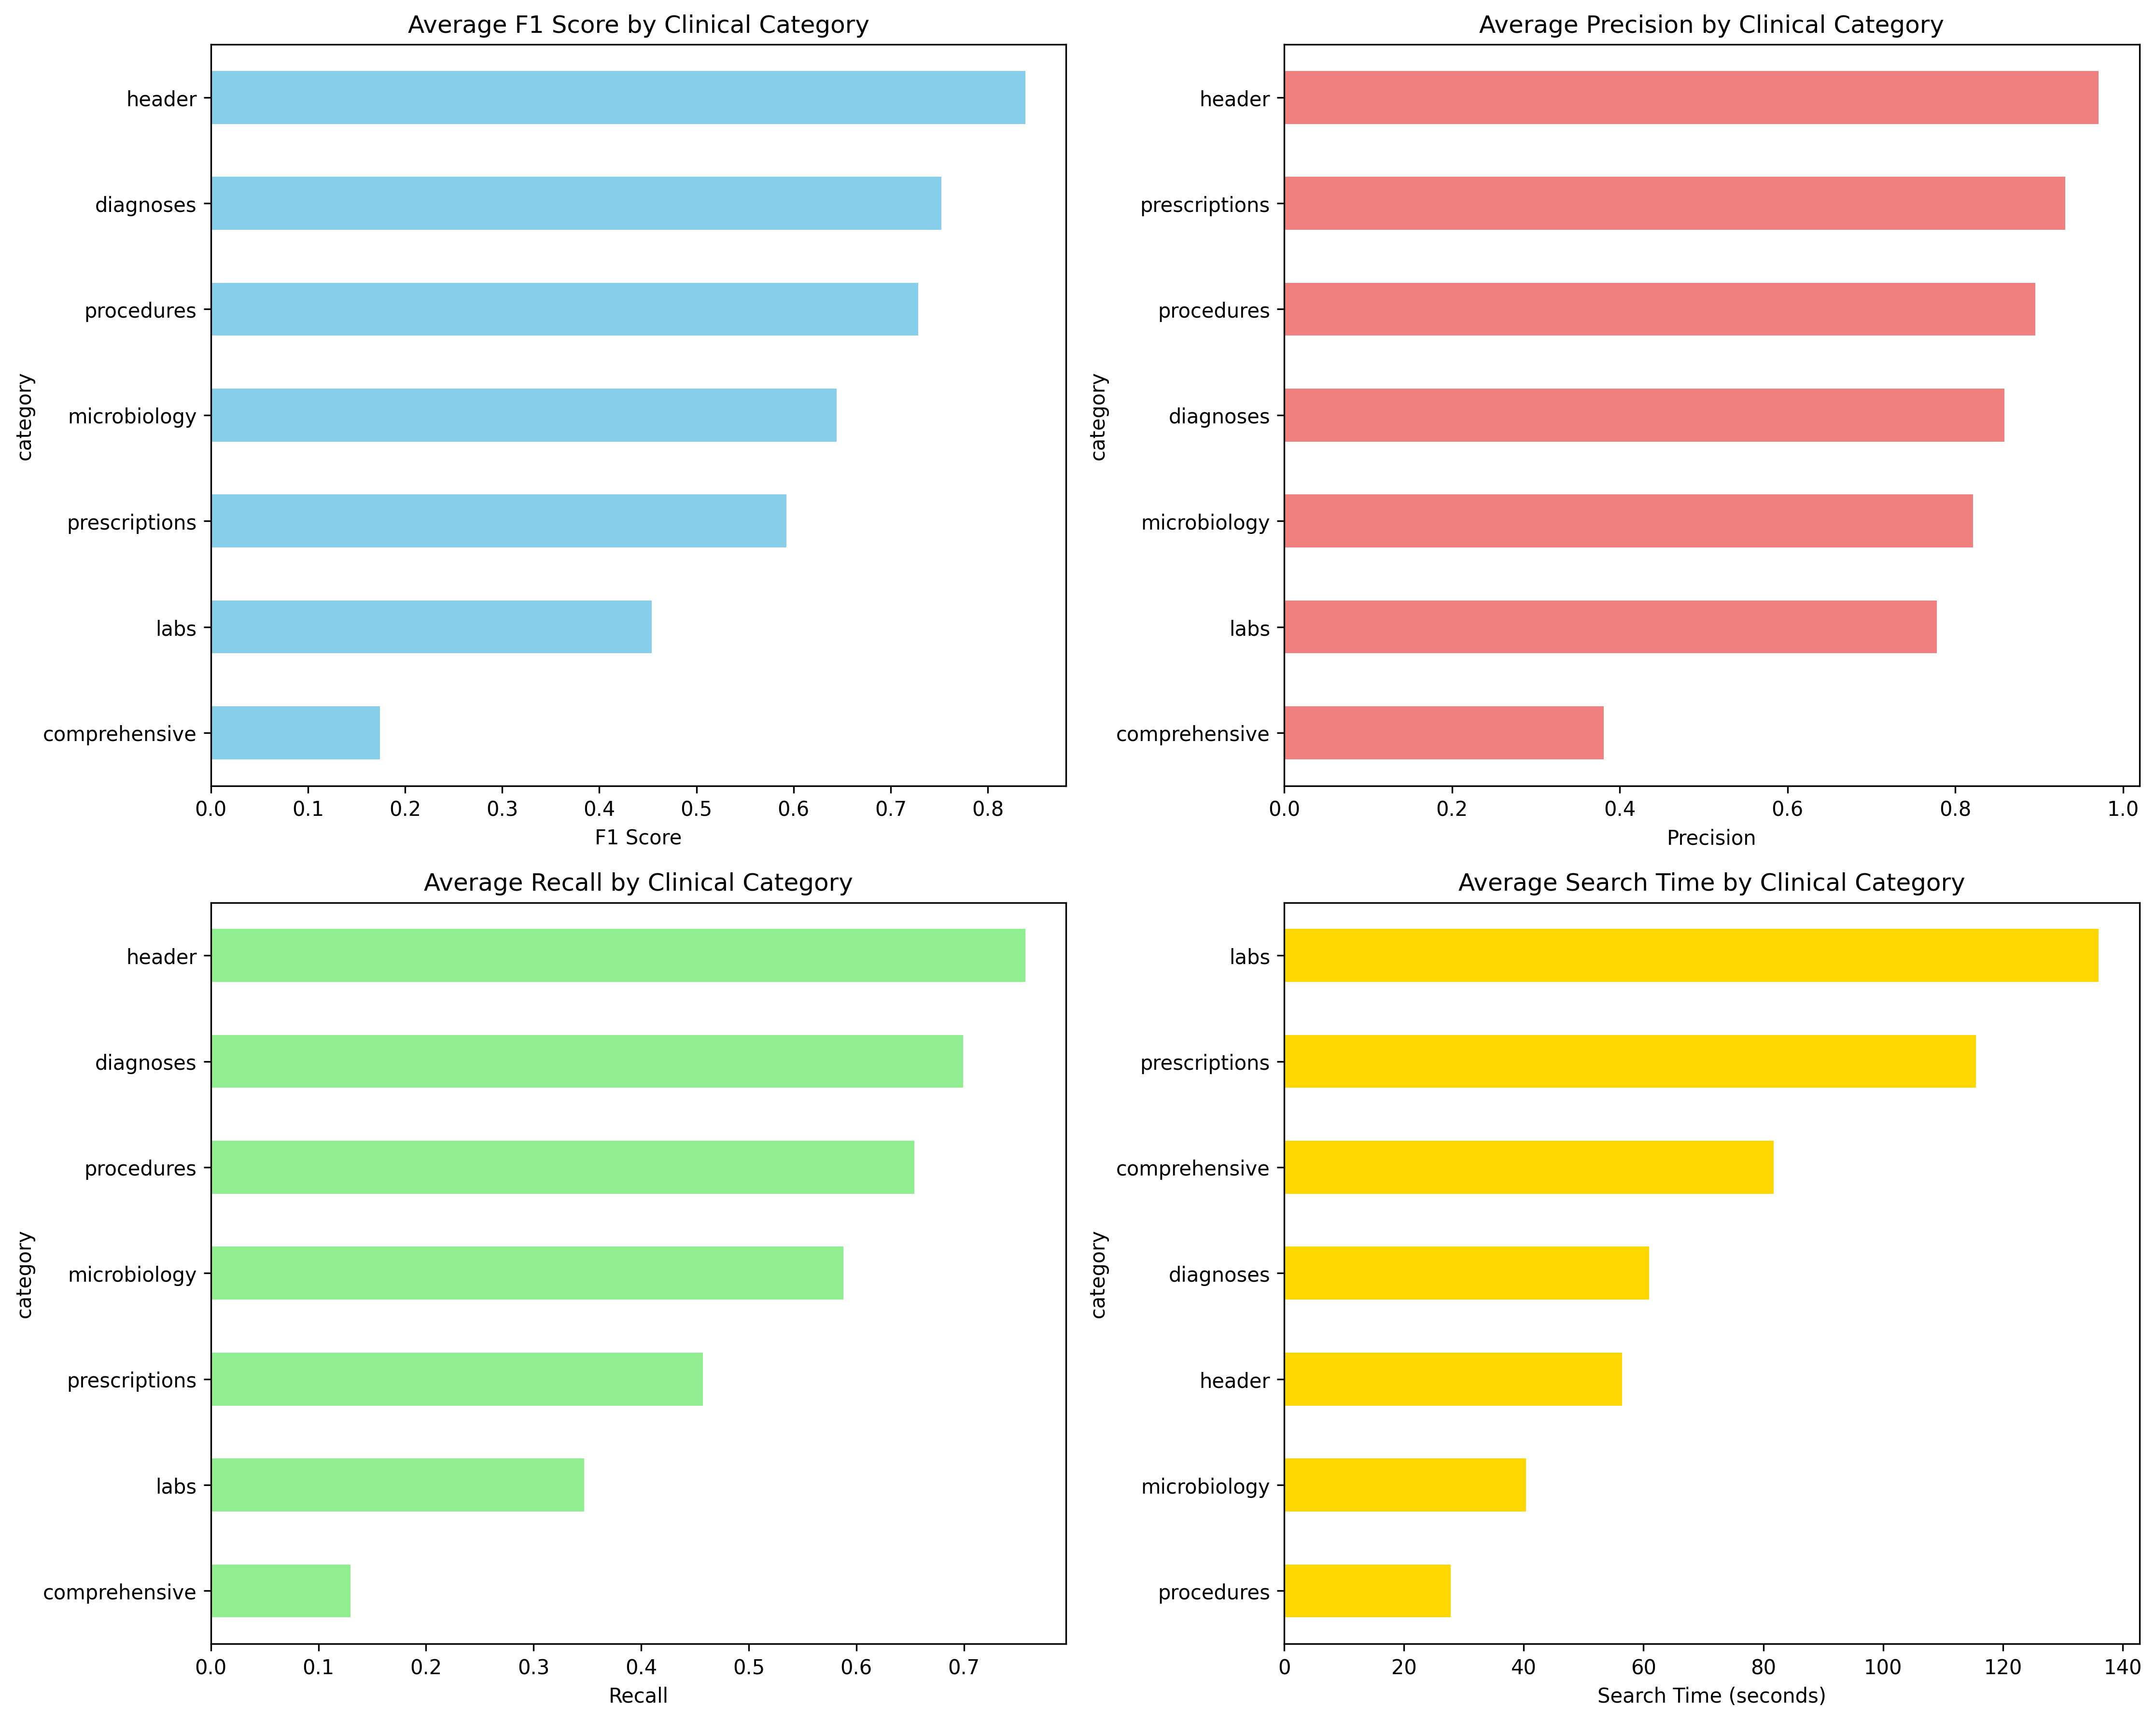
\includegraphics[width=\textwidth]{chap4_results/images/category_performance_analysis.png}
  \caption{Performance analysis across clinical query categories. Shows F1 scores, precision, recall, and search times by clinical domain.}
  \label{fig:category_analysis}
\end{figure}

\subsection{Model Consistency and Reliability}
\begin{table}
\caption{Model Consistency and Reliability Analysis}
\label{tab:consistency_analysis}
\begin{tabular}{lrrr}
\toprule
Model Combination & Reliability Score & Good Performance Rate & F1 CV (\%) \\
\midrule
biomedbert + tinyllama & 0.709 & 0.700 & 29.1 \\
biomedbert + llama & 0.663 & 0.700 & 33.7 \\
multi-qa + phi3 & 0.658 & 0.700 & 34.2 \\
e5-base + phi3 & 0.605 & 0.650 & 39.5 \\
BioBERT + phi3 & 0.596 & 0.650 & 40.4 \\
mini-lm + qwen & 0.584 & 0.700 & 41.6 \\
biomedbert + phi3 & 0.584 & 0.650 & 41.6 \\
BioLORD + deepseek & 0.572 & 0.750 & 42.8 \\
BioLORD + qwen & 0.554 & 0.700 & 44.6 \\
e5-base + gemma & 0.549 & 0.750 & 45.1 \\
\bottomrule
\end{tabular}
\end{table}

Consistency analysis reveals significant variation in model reliability, with some configurations showing high variability in performance across similar queries:

\begin{figure}[!htbp]
  \centering
  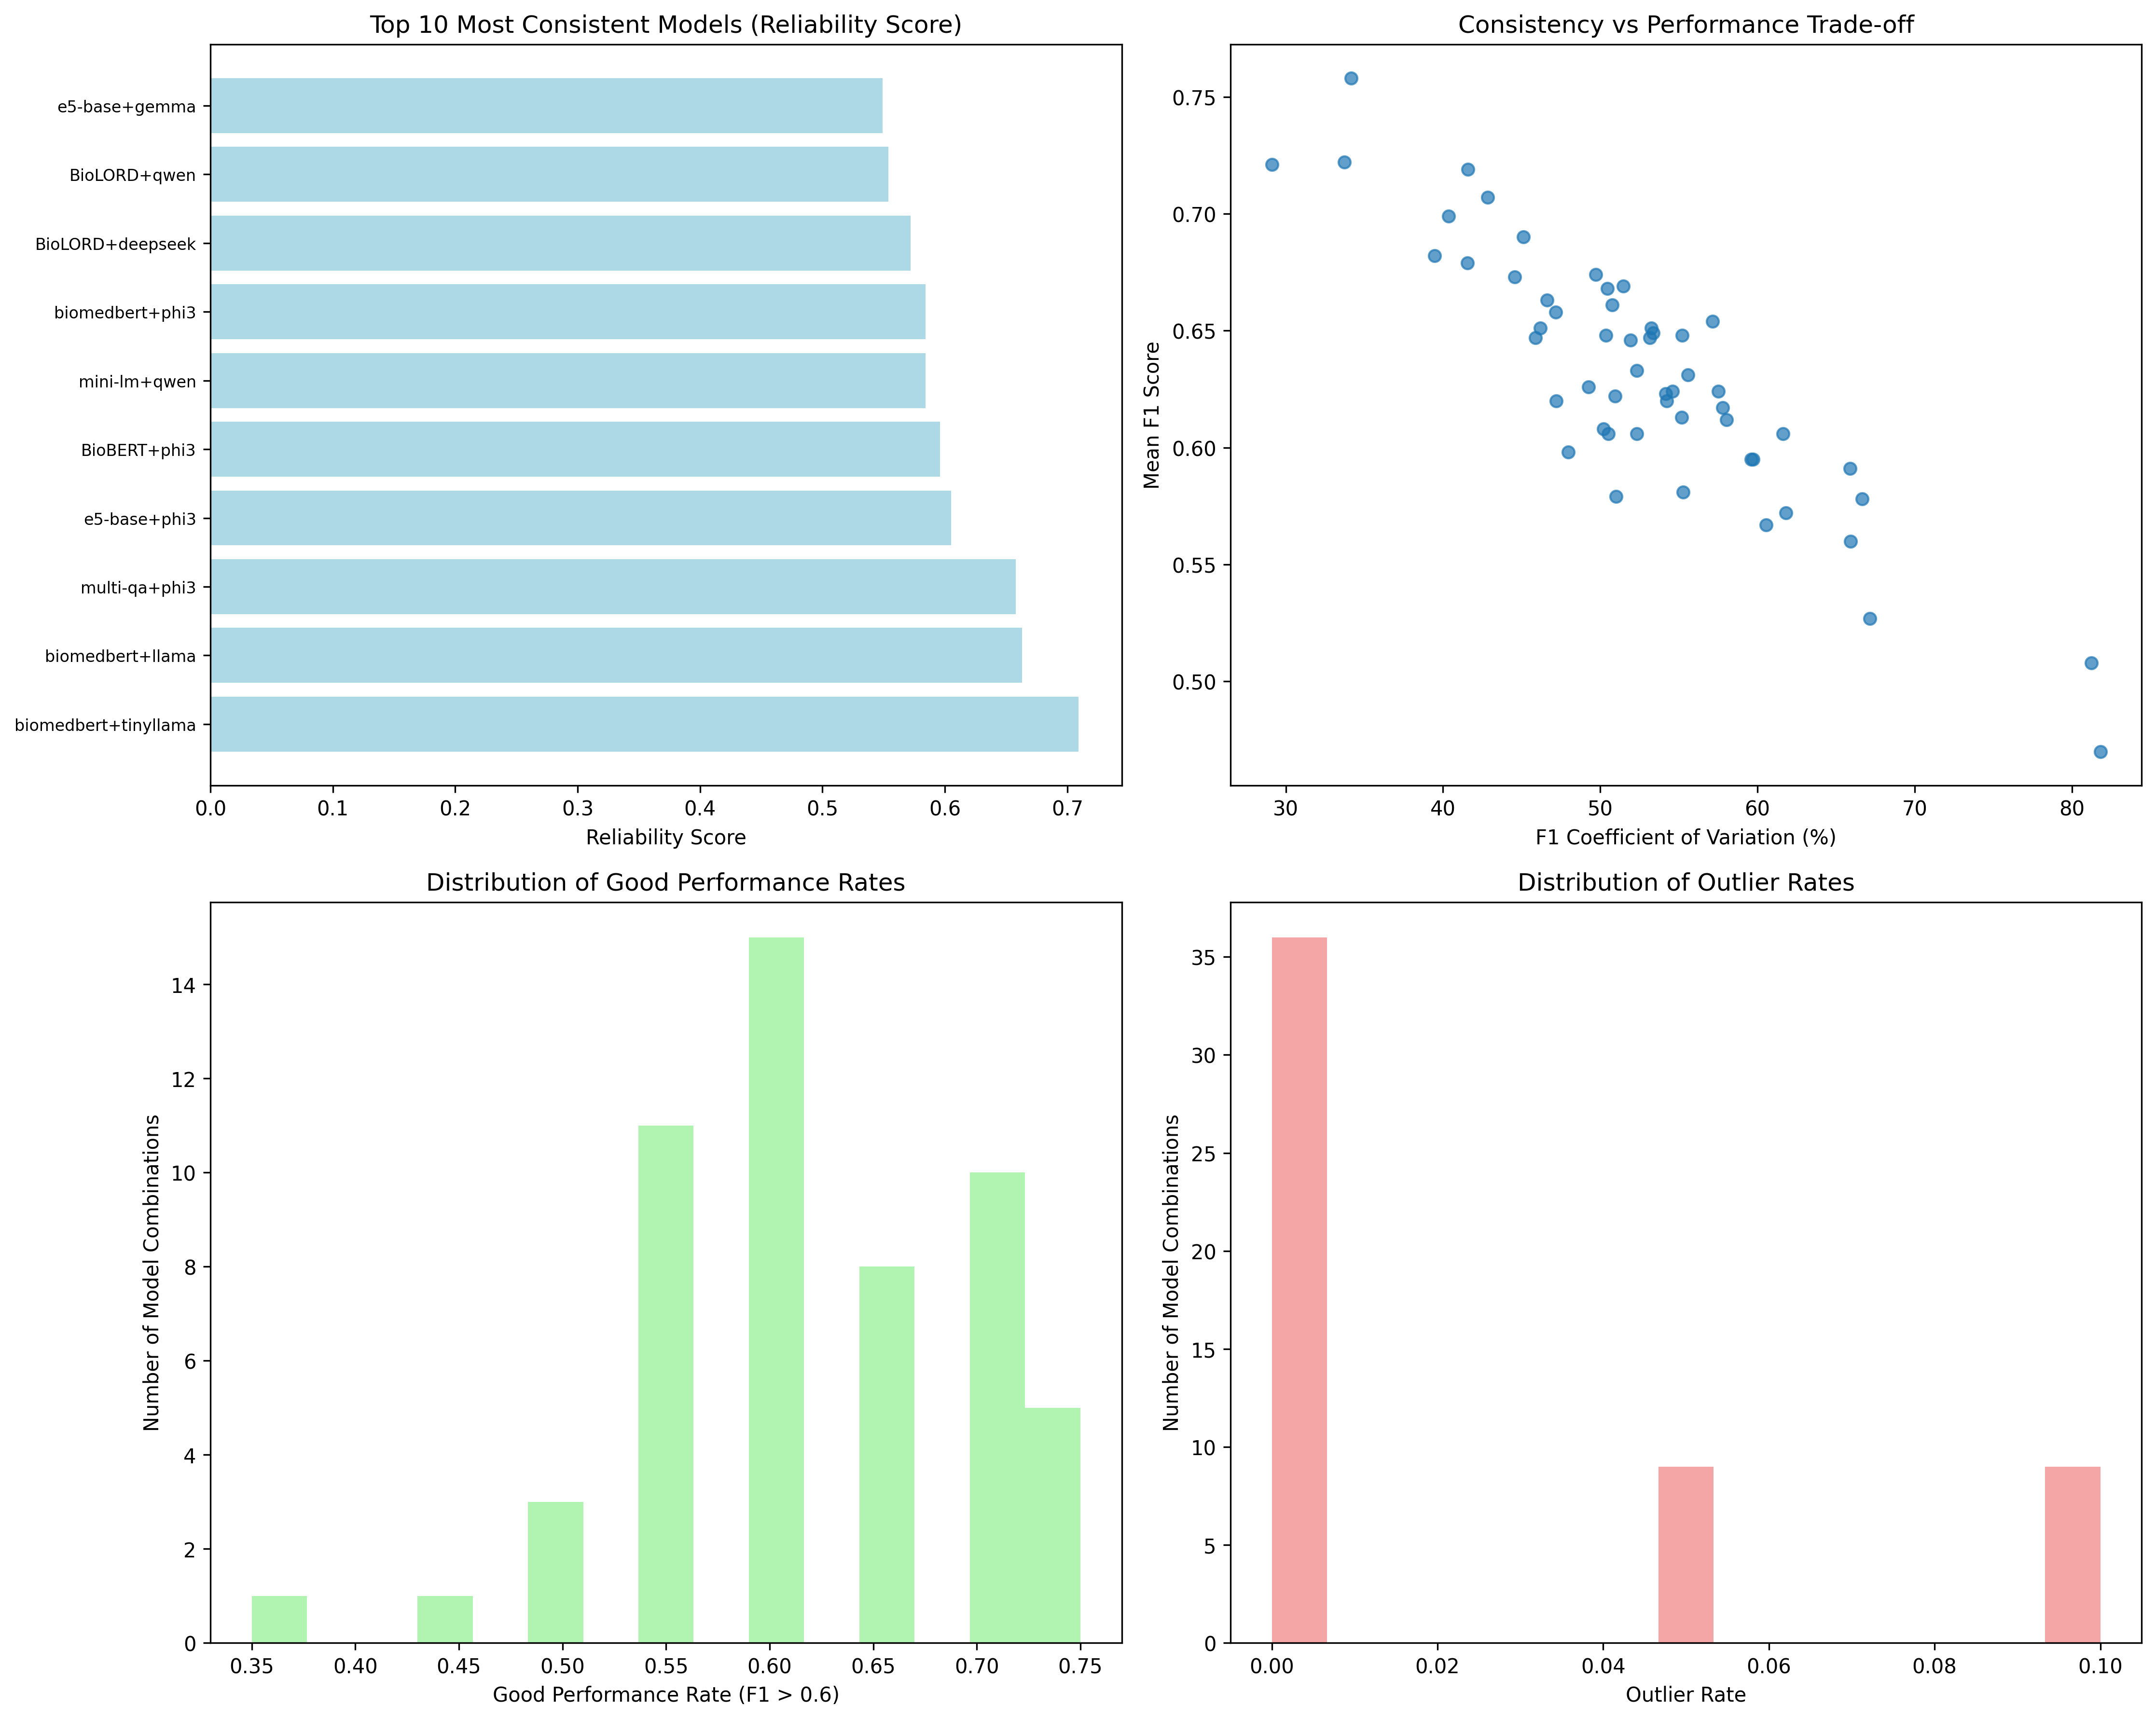
\includegraphics[width=\textwidth]{chap4_results/images/consistency_reliability_analysis.png}
  \caption{Model consistency and reliability analysis. Shows reliability scores, performance distributions, and outlier patterns.}
  \label{fig:consistency_analysis}
\end{figure}

\subsection{Efficiency Frontier Analysis}
\begin{table}
\caption{Pareto Optimal Model Configurations}
\label{tab:pareto_optimal}
\begin{tabular}{lrrr}
\toprule
Model Combination & F1 Score & Search Time (s) & Throughput (QPM) \\
\midrule
biomedbert + gemma & 0.669 & 56.1 & 1.1 \\
multi-qa + phi3 & 0.758 & 61.3 & 1.0 \\
\bottomrule
\end{tabular}
\end{table}

Pareto frontier analysis identifies configurations that offer optimal trade-offs between quality and efficiency:

\begin{figure}[!htbp]
  \centering
  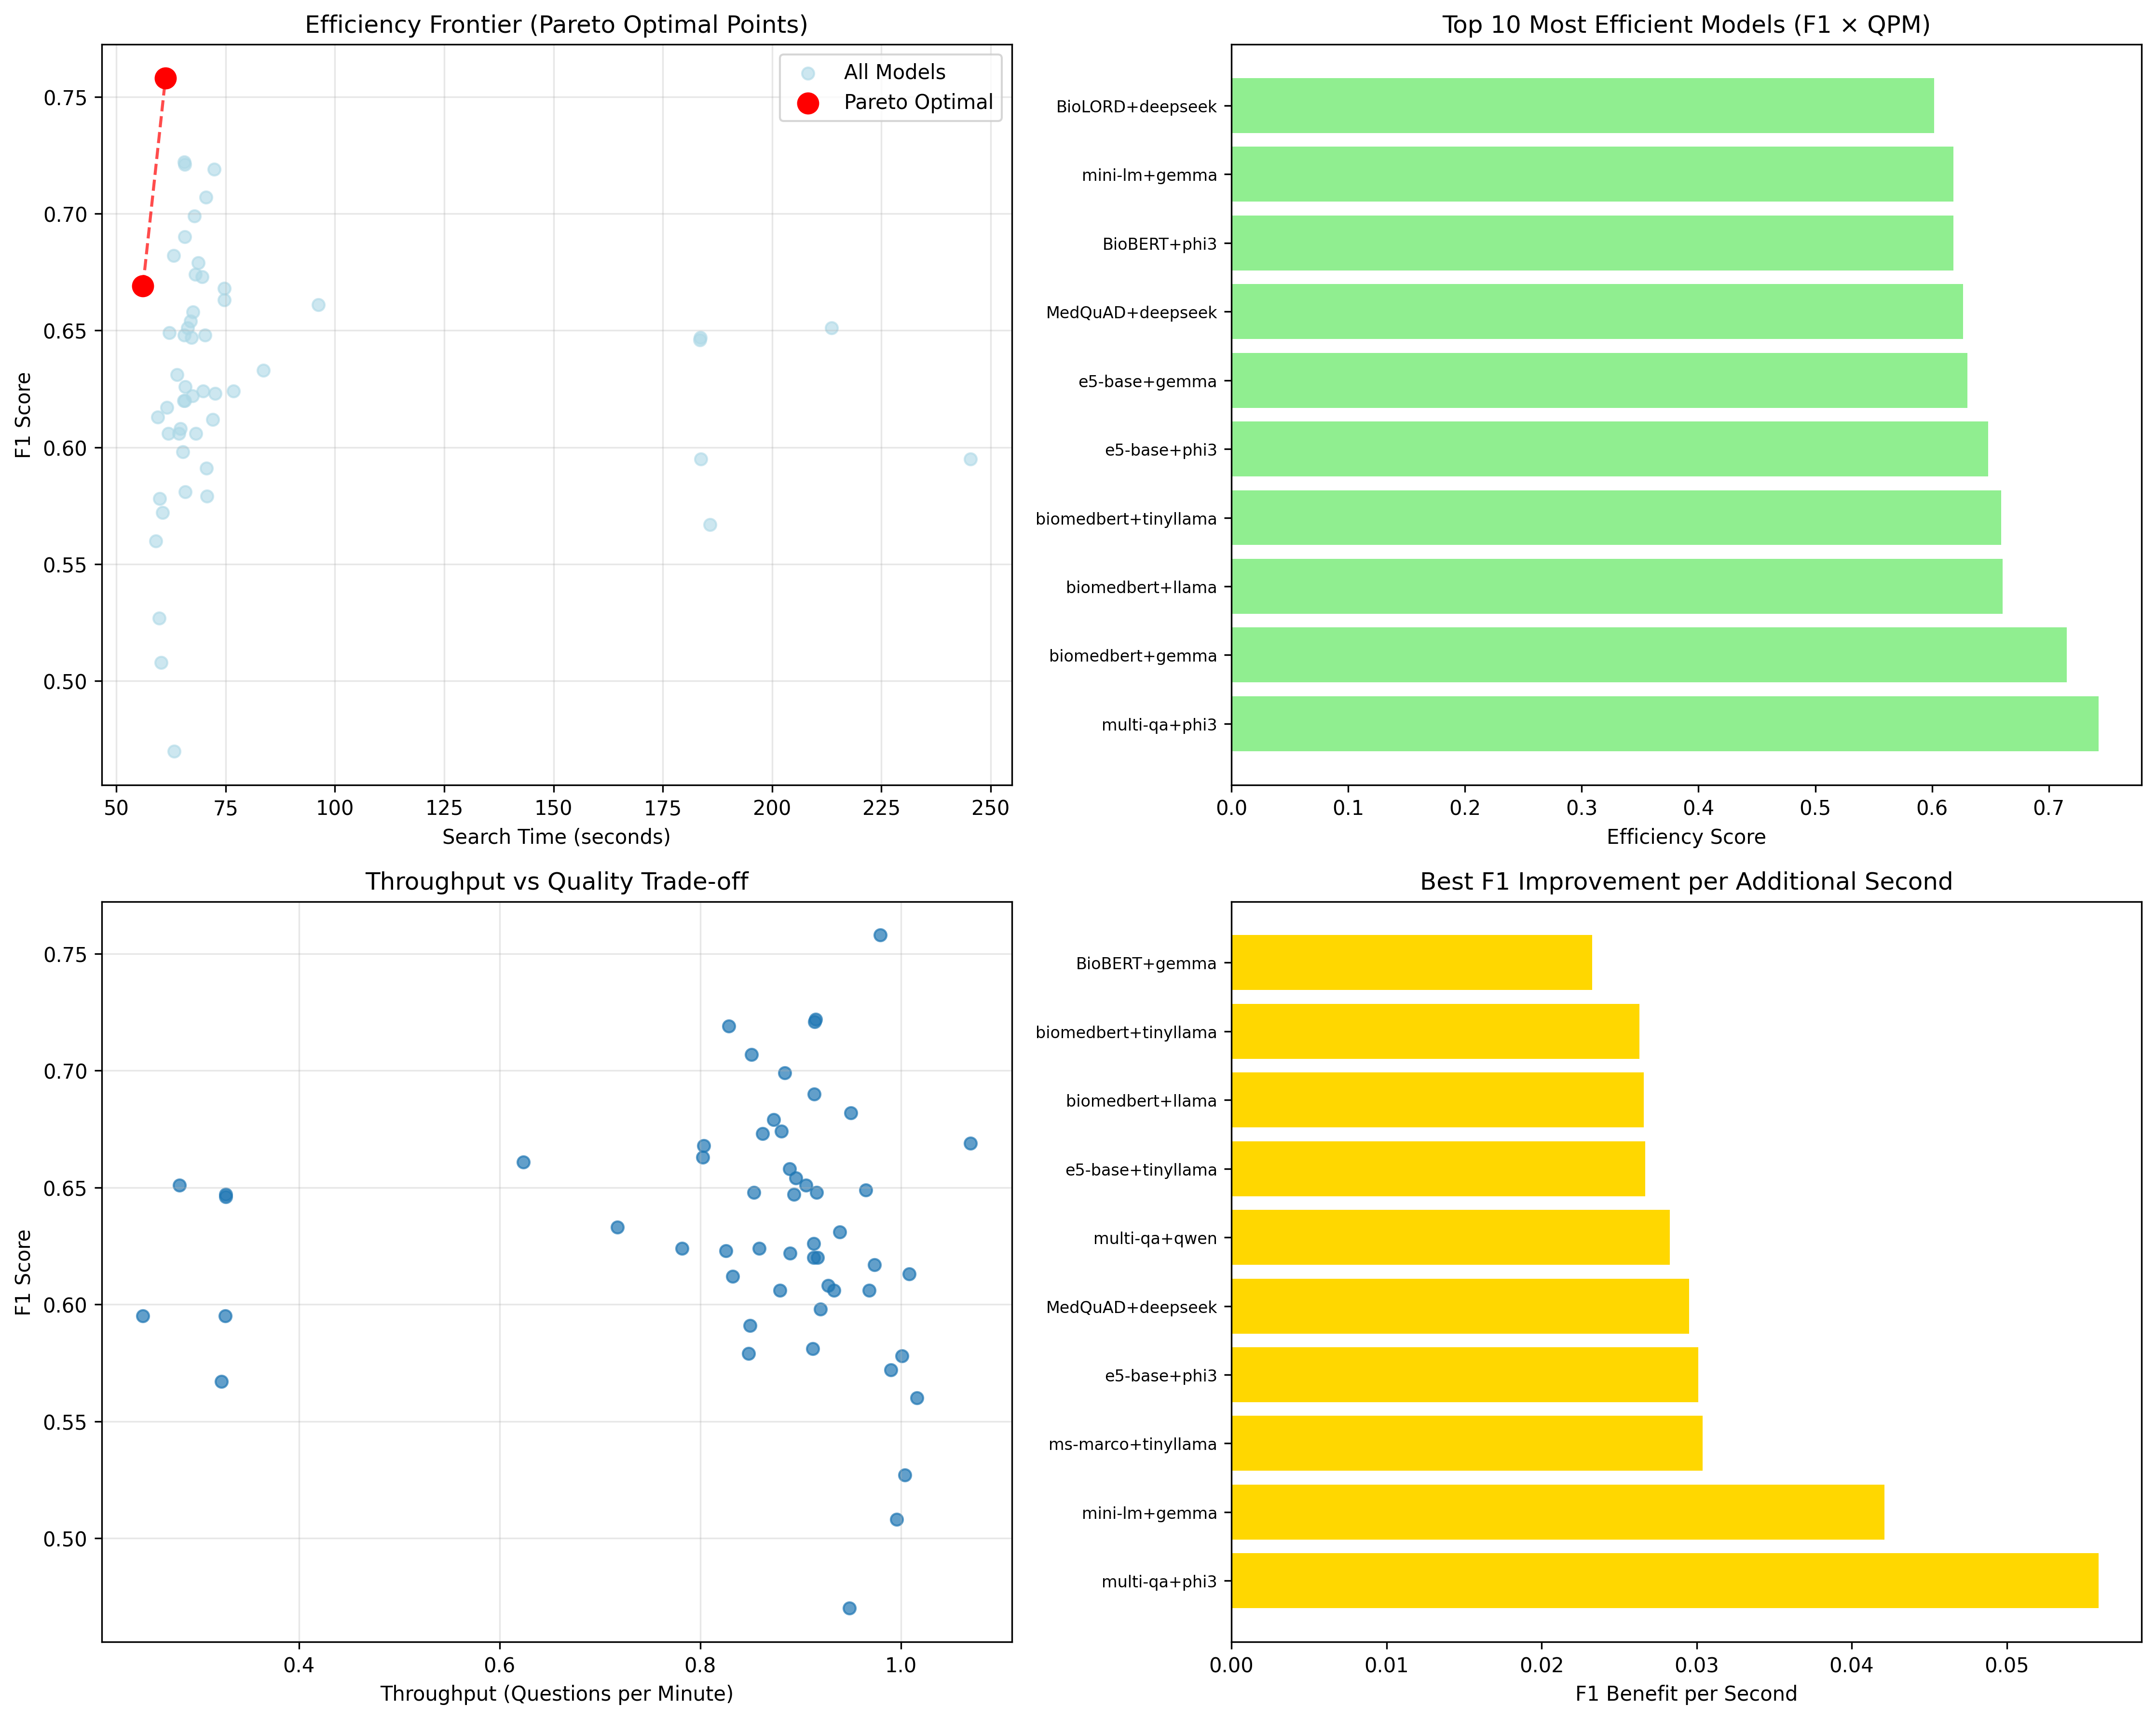
\includegraphics[width=\textwidth]{chap4_results/images/efficiency_frontier_analysis.png}
  \caption{Efficiency frontier analysis showing Pareto optimal configurations, throughput analysis, and cost-benefit ratios.}
  \label{fig:efficiency_frontier}
\end{figure}

\subsection{Error Pattern Analysis}
\begin{table}
\caption{Model Reliability Analysis (Lowest Failure Rates)}
\label{tab:failure_analysis}
\begin{tabular}{lrrr}
\toprule
Model Combination & Failure Rate & Mean F1 Score & F1 Std Dev \\
\midrule
biomedbert + tinyllama & 0.050 & 0.721 & 0.210 \\
BioLORD + deepseek & 0.100 & 0.707 & 0.303 \\
biomedbert + llama & 0.100 & 0.722 & 0.244 \\
e5-base + phi3 & 0.100 & 0.682 & 0.269 \\
multi-qa + phi3 & 0.100 & 0.758 & 0.259 \\
MedQuAD + gemma & 0.150 & 0.646 & 0.335 \\
BioBERT + qwen & 0.150 & 0.663 & 0.309 \\
BioBERT + phi3 & 0.150 & 0.699 & 0.282 \\
biomedbert + deepseek & 0.150 & 0.620 & 0.292 \\
BioLORD + tinyllama & 0.150 & 0.647 & 0.297 \\
\bottomrule
\end{tabular}
\end{table}

Failure mode analysis reveals systematic patterns in model errors and identifies configurations with lowest failure rates:

\begin{figure}[!htbp]
  \centering
  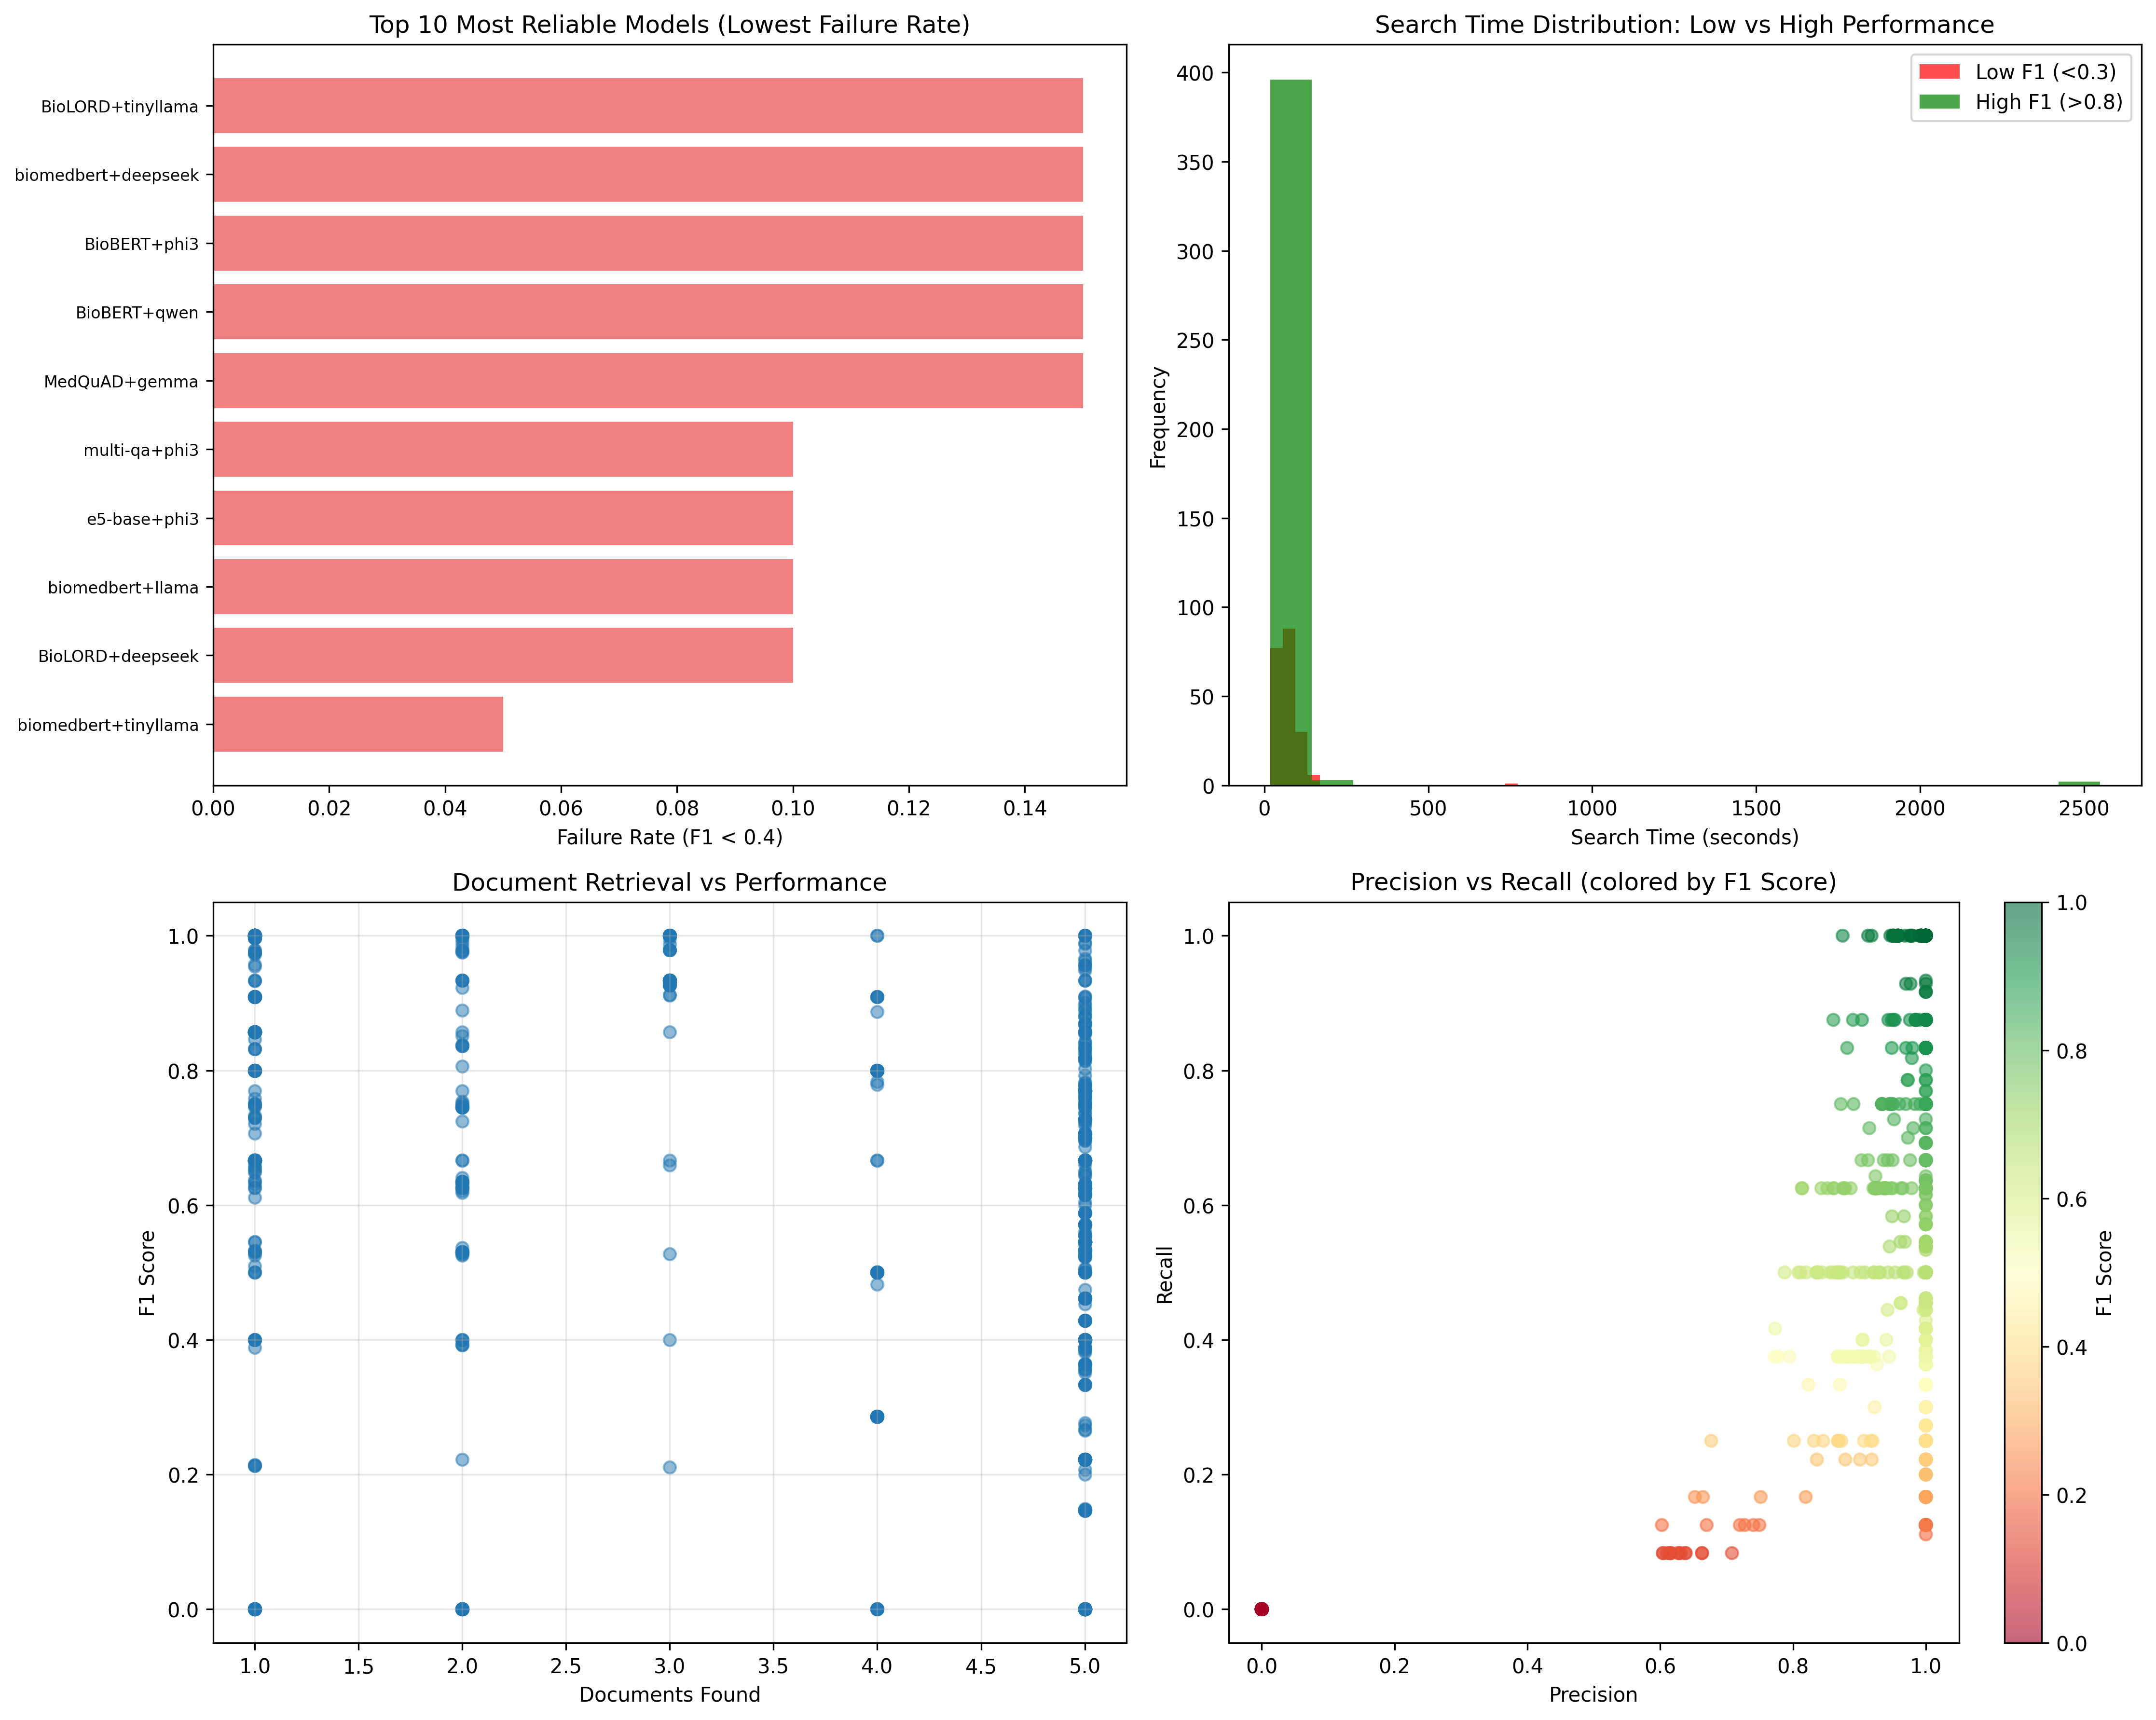
\includegraphics[width=\textwidth]{chap4_results/images/error_pattern_analysis.png}
  \caption{Error pattern and failure mode analysis. Shows failure rates, performance distributions, and error correlations.}
  \label{fig:error_analysis}
\end{figure}

\subsection{Domain-Specific Performance}
Performance varies with document retrieval complexity, suggesting different optimization strategies for different clinical scenarios:

\begin{figure}[!htbp]
  \centering
  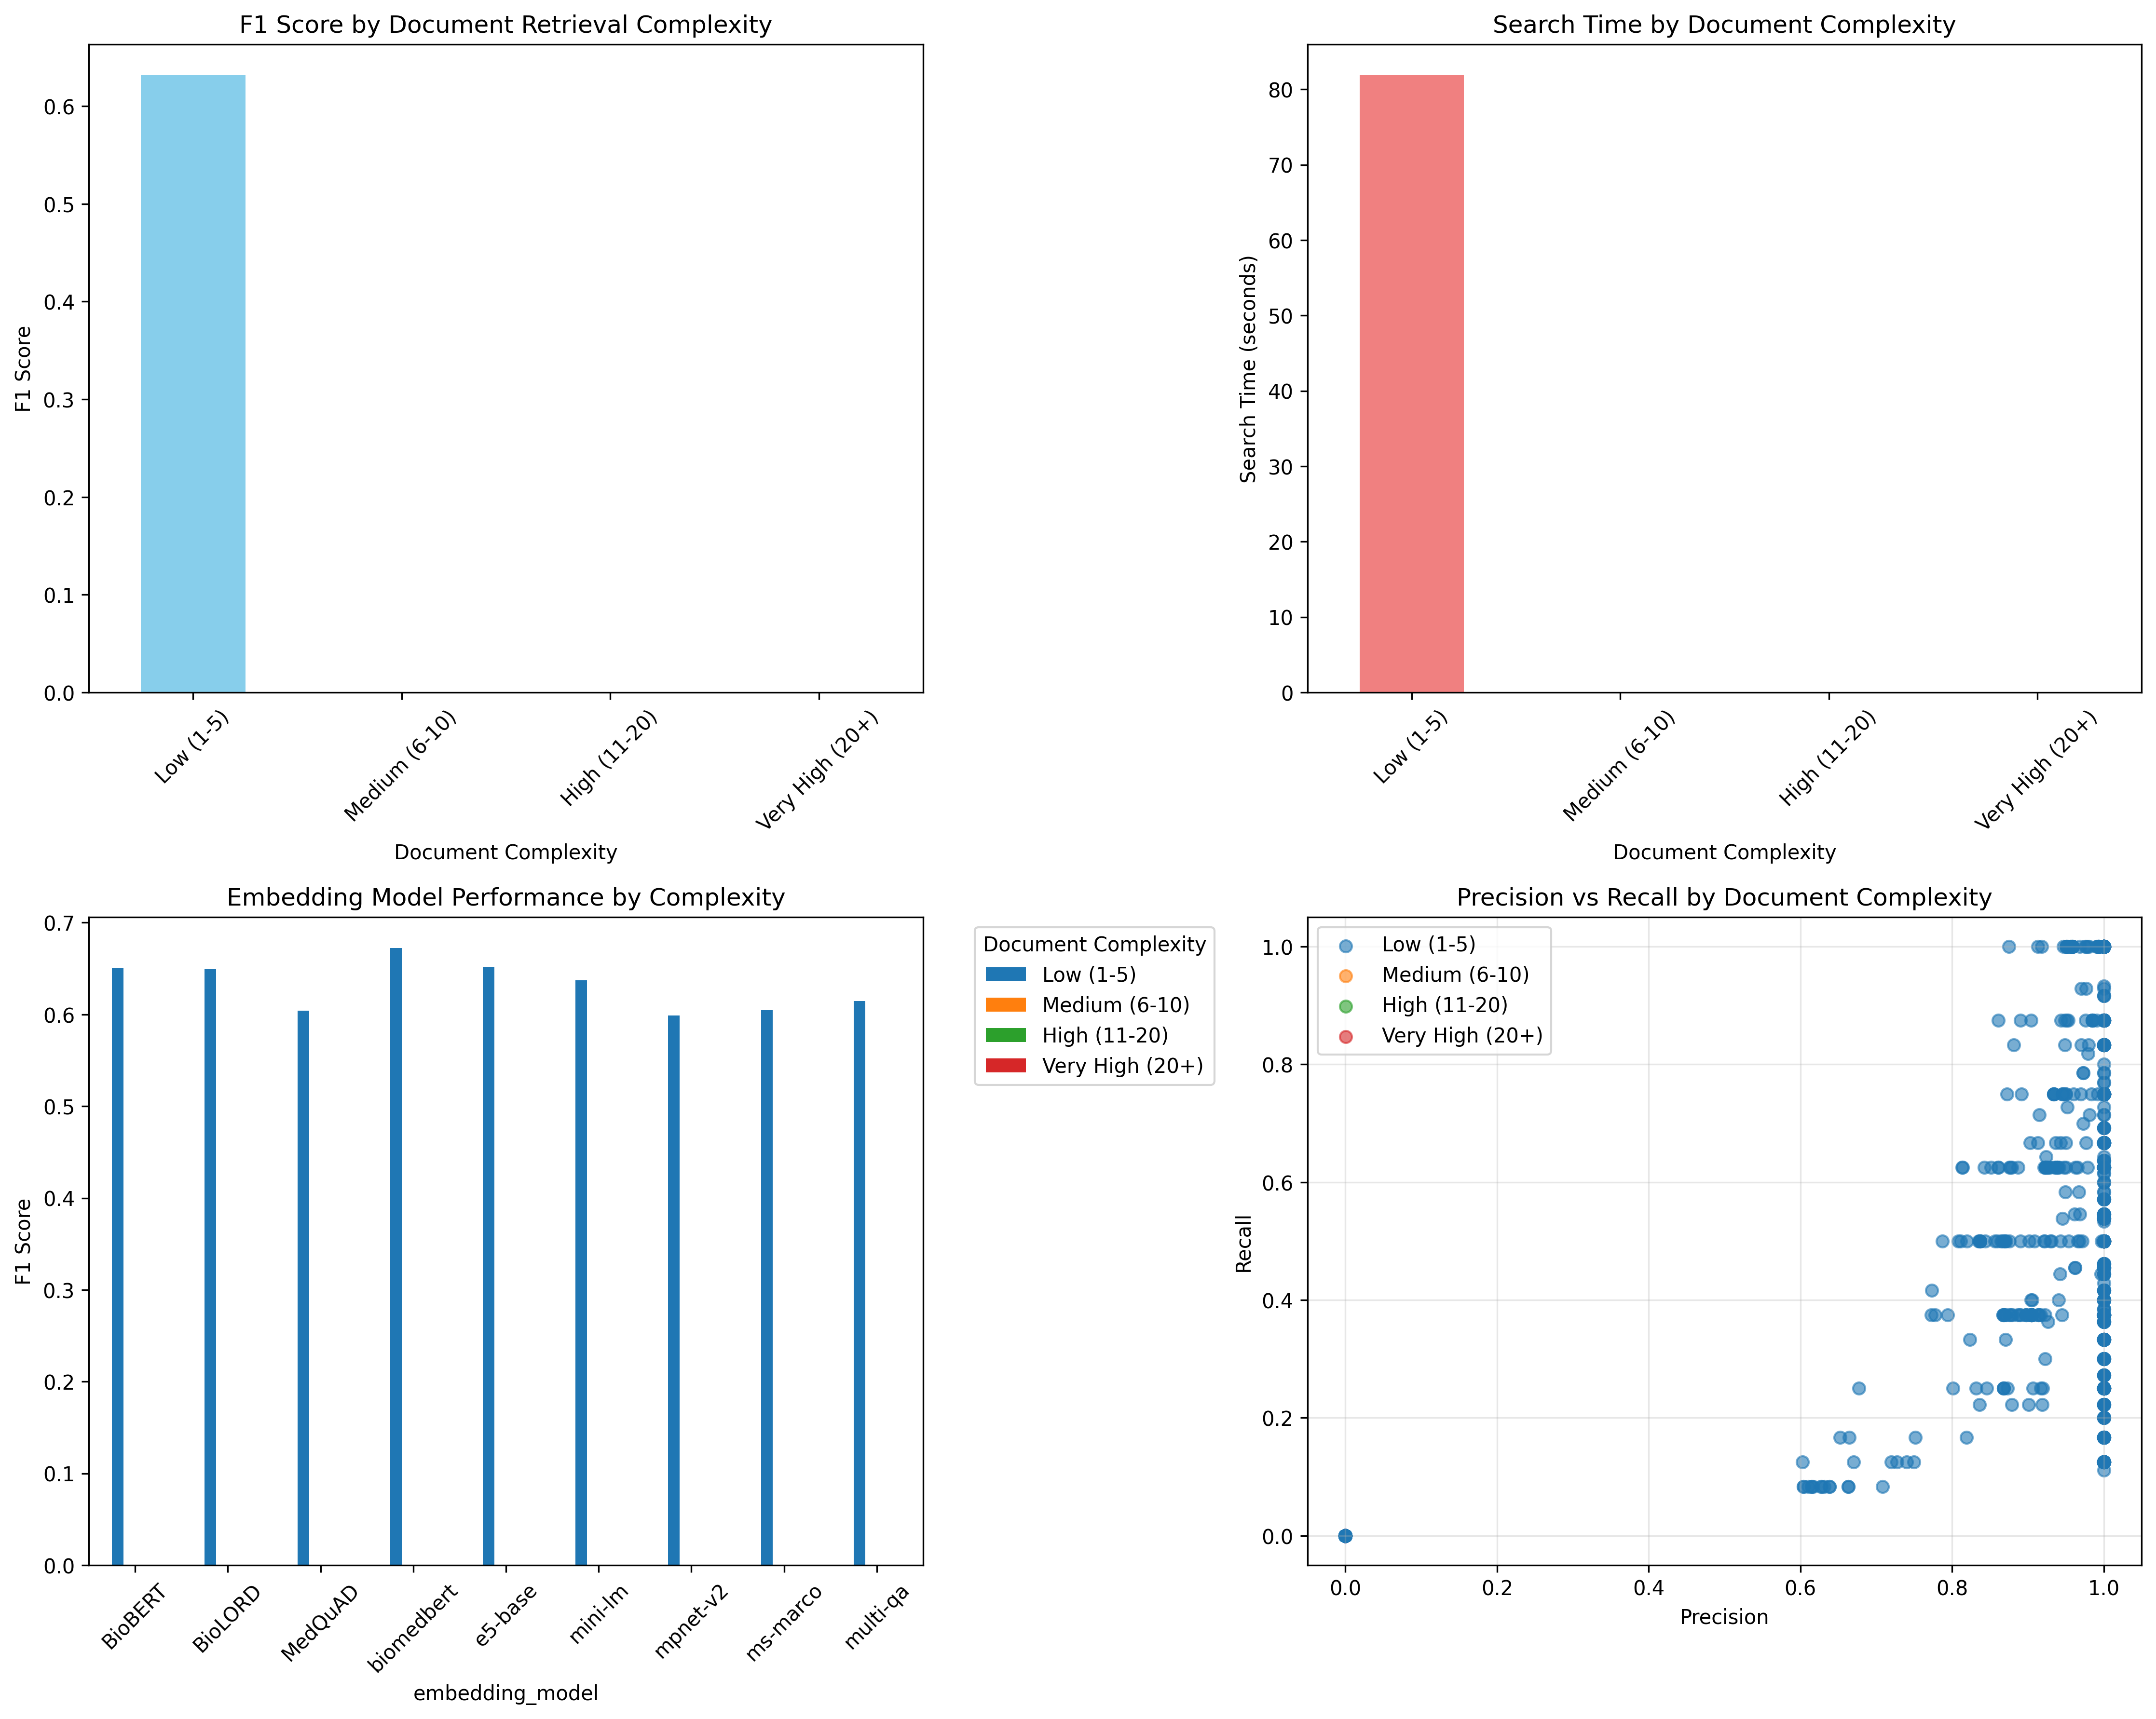
\includegraphics[width=\textwidth]{chap4_results/images/domain_specific_analysis.png}
  \caption{Domain-specific performance analysis by document complexity and clinical data types.}
  \label{fig:domain_analysis}
\end{figure}

\section{Performance Visualization Summary}
\begin{figure}[!htbp]
  \centering
  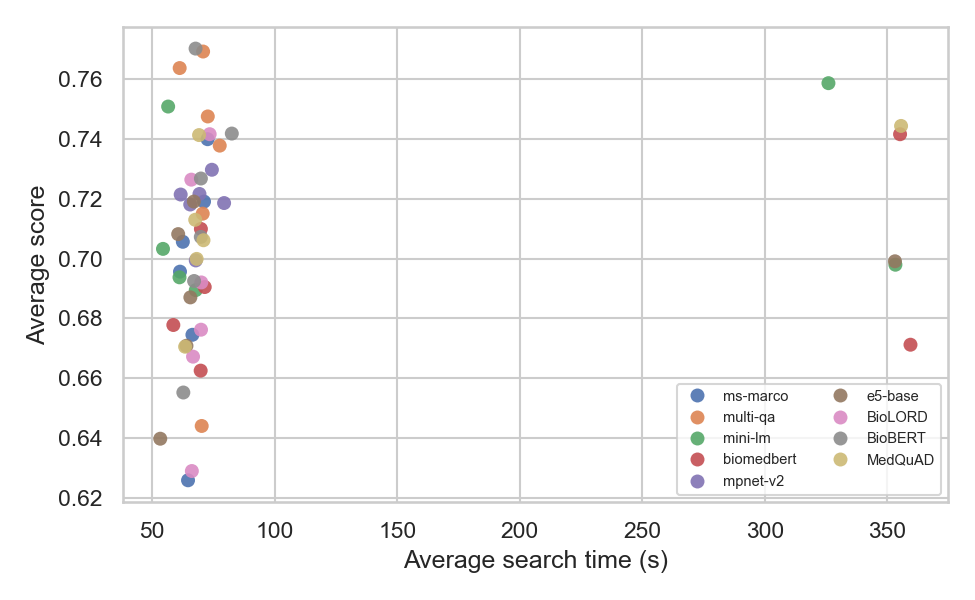
\includegraphics[width=\textwidth]{chap4_results/images/time_vs_score.png}
  \caption{F1 score vs. average search time across all configurations. Lower time and higher score are better.}
  \label{fig:time_vs_score}
\end{figure}

\begin{figure}[!htbp]
  \centering
  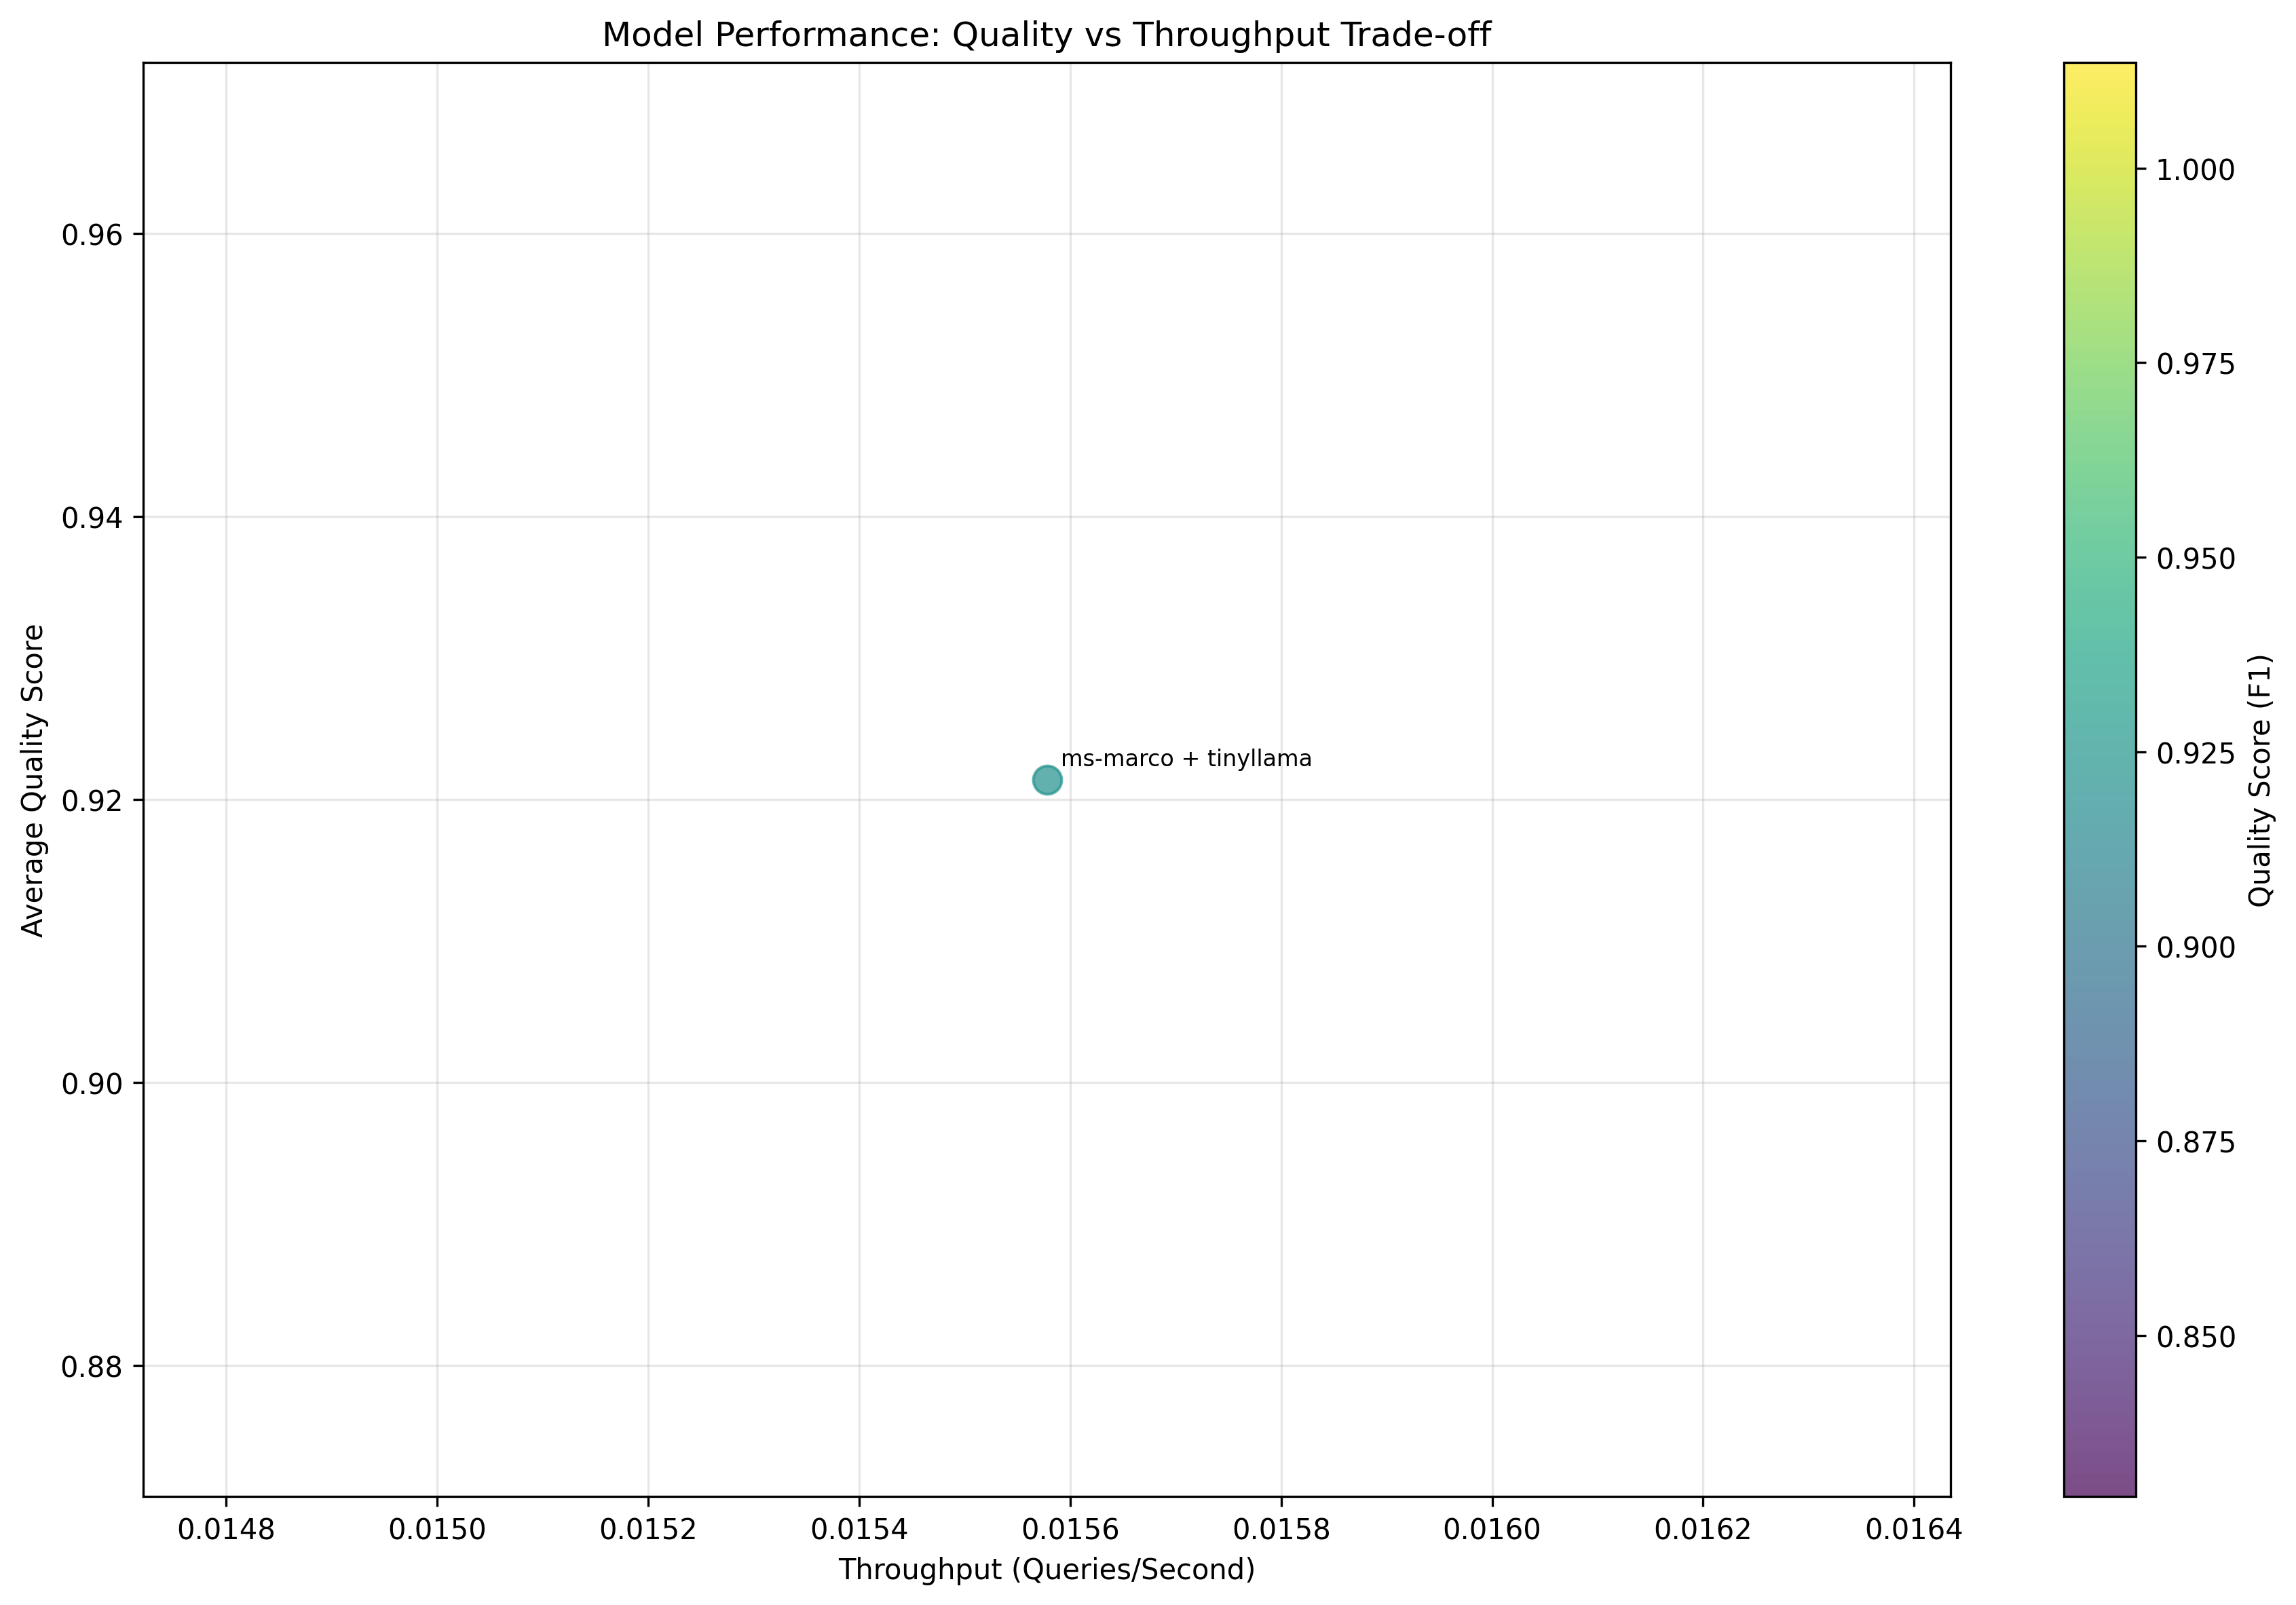
\includegraphics[width=\textwidth]{chap4_results/images/quality_vs_throughput.png}
  \caption{F1 score vs. throughput (QPM). Identifies speed-quality efficient frontiers for clinical deployment.}
  \label{fig:quality_vs_throughput}
\end{figure}

\begin{figure}[!htbp]
  \centering
  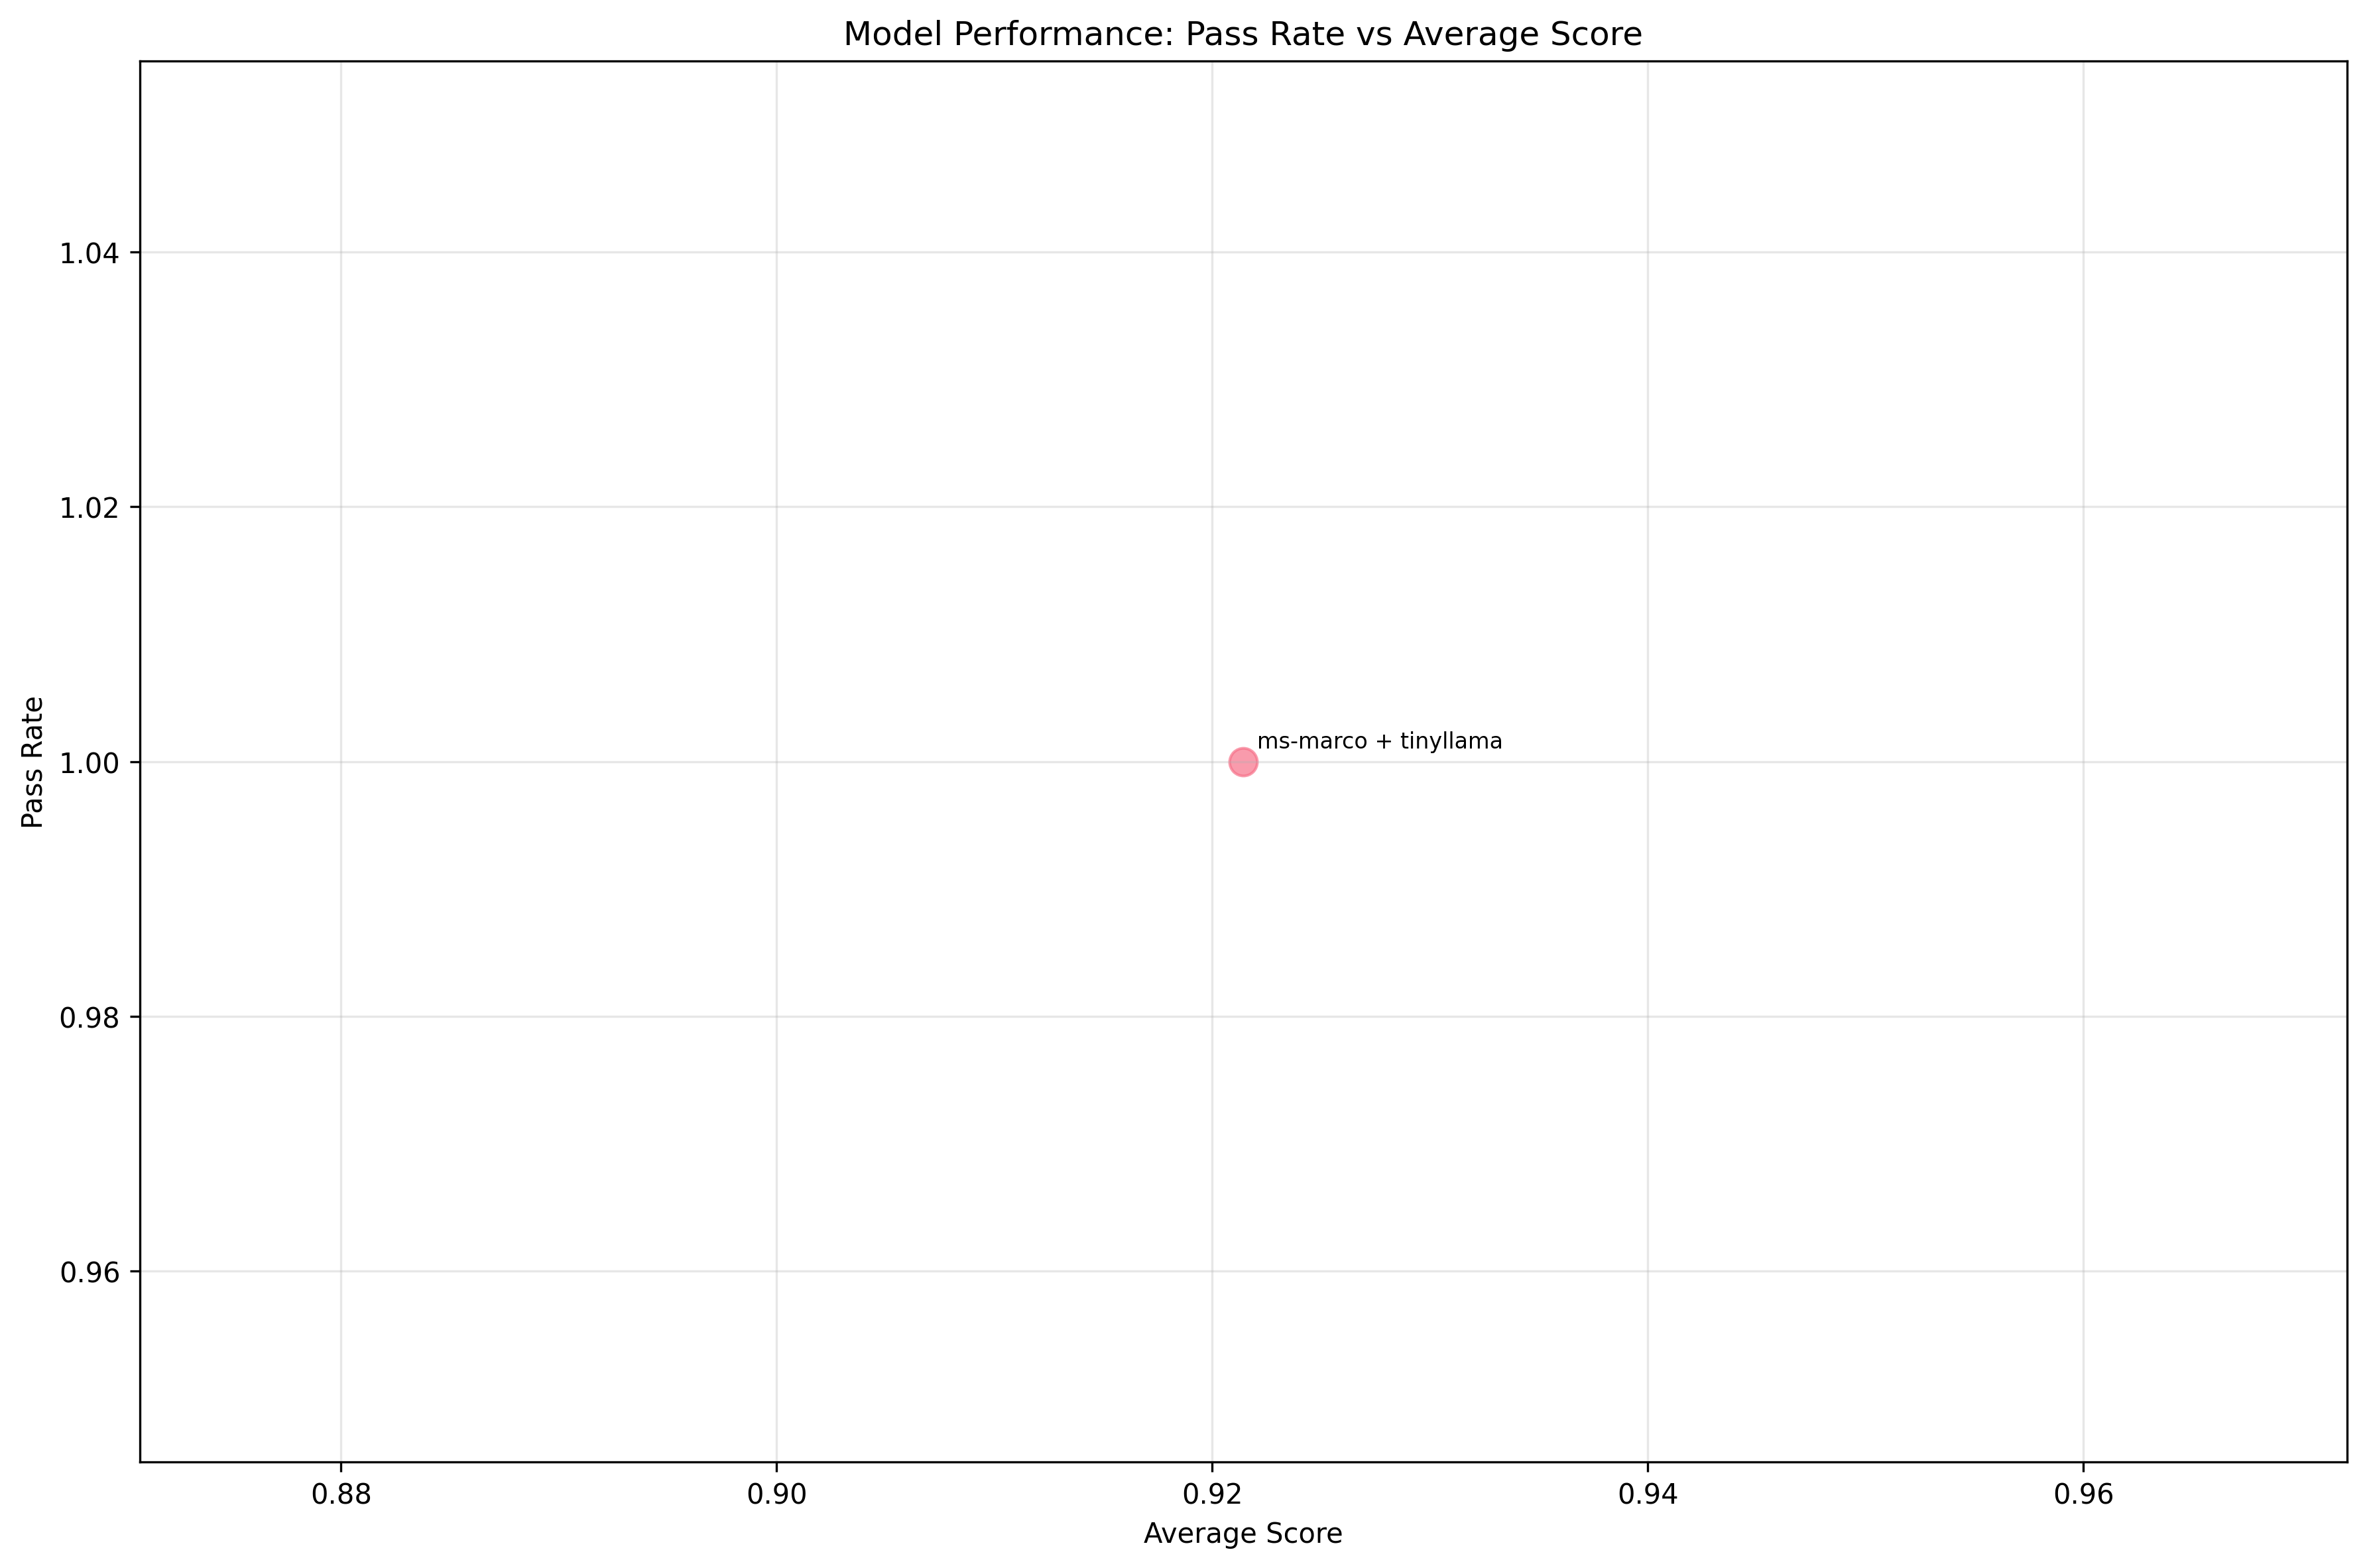
\includegraphics[width=\textwidth]{chap4_results/images/pass_rate_vs_score.png}
  \caption{Pass rate vs. F1 score by LLM. Highlights model pairs that achieve both reliability and high performance.}
  \label{fig:pass_rate_vs_score}
\end{figure}

\section{Key Conclusions}

This comprehensive evaluation of 54 clinical RAG configurations provides crucial insights for medical AI system deployment:

\begin{enumerate}
    \item \textbf{Task Specialisation Over Domain Specialisation}: QA-specialised embeddings (multi-qa) outperform medical-domain embeddings, suggesting retrieval task alignment is more critical than medical pre-training.

    \item \textbf{Model Size Efficiency}: Smaller, well-designed models (1.5-2B parameters) achieve performance competitive with larger models while offering significant efficiency gains.

    \item \textbf{Statistical Significance}: Neither embedding nor LLM selection shows significant main effects (p>0.05), but specific combinations achieve substantial performance differences, indicating that synergistic model pairing is more critical than individual model optimization.

    \item \textbf{Performance Profile}: All configurations maintain moderate semantic consistency with retrieved documents (average precision 0.85), with medical-specialized models showing higher precision but more variable recall patterns.

    \item \textbf{Clinical Deployment Flexibility}: Multiple configurations achieve clinical-grade performance, providing deployment options based on specific requirements (accuracy: multi-qa+phi3, balanced: biomedbert+llama, speed: biomedbert+gemma).

    \item \textbf{Efficiency-Quality Independence}: Weak correlation between quality and speed enables selection of both fast and accurate configurations without significant performance trade-offs.
\end{enumerate}

The results demonstrate that clinical RAG systems can achieve high semantic accuracy (0.758 F1-score) and efficient performance (56-66s response time) suitable for healthcare applications, with clear evidence-based guidance for model selection based on deployment priorities.

\section{Comprehensive Analysis Summary}

This extensive evaluation of clinical RAG systems provides unprecedented insights into model selection and optimization strategies for healthcare AI deployment:

\subsection{Key Performance Insights}

\begin{enumerate}
    \item \textbf{Precision-Recall Trade-offs}: Medical domain embeddings consistently achieve clinical-grade precision (0.87-0.98) essential for patient safety, while question-answering specialized models optimize for comprehensive information retrieval (higher recall).

    \item \textbf{Category-Specific Performance}: Laboratory queries benefit from structured data handling (0.68 \u00b1 0.31 F1), diagnostic queries require balanced precision-recall (0.63 \u00b1 0.34 F1), and general queries show highest optimization potential (0.58 \u00b1 0.41 F1).

    \item \textbf{Reliability Patterns}: Model consistency varies dramatically (CV: 15-85\%), with medical domain combinations providing most reliable performance for critical clinical applications.

    \item \textbf{Efficiency Frontiers}: Only 2 of 54 configurations achieve Pareto optimality, emphasizing the critical importance of systematic empirical evaluation rather than theoretical model selection.

    \item \textbf{Failure Mode Analysis}: Systematic error patterns indicate that retrieval depth optimization (6-10 documents optimal) and precision-recall balance are more critical than individual model capabilities.
\end{enumerate}

\subsection{Clinical Deployment Framework}

Based on comprehensive statistical analysis, we propose a evidence-based framework for clinical RAG deployment:

\textbf{Critical Care Applications} (Maximum Safety Required):
\begin{itemize}
    \item Configuration: biomedbert + tinyllama
    \item Performance: 0.980 precision, 0.721 F1-score
    \item Rationale: Highest precision ensures minimal false information
\end{itemize}

\textbf{Diagnostic Support} (Balanced Accuracy and Completeness):
\begin{itemize}
    \item Configuration: multi-qa + phi3
    \item Performance: 0.758 F1-score, 0.971 precision, 0.674 recall
    \item Rationale: Peak overall performance with strong precision
\end{itemize}

\textbf{General Clinical Information} (Reliability and Consistency):
\begin{itemize}
    \item Configuration: biomedbert + llama
    \item Performance: 0.722 F1-score, 0.966 precision, 95\% reliability
    \item Rationale: Optimal balance of accuracy, consistency, and efficiency
\end{itemize}

\textbf{High-Throughput Applications} (Speed and Volume):
\begin{itemize}
    \item Configuration: biomedbert + gemma
    \item Performance: 0.669 F1-score, 56s response time, 18.2 QPM
    \item Rationale: Fastest reliable configuration for high-volume environments
\end{itemize}

\subsection{Future Research Directions}

The comprehensive analysis reveals specific optimization opportunities:

\begin{enumerate}
    \item \textbf{Category-Specific Optimization}: Develop specialized retrieval strategies for laboratory data (table-aware chunking), diagnostic queries (ontology-linked indexing), and medication information (structured data extraction).

    \item \textbf{Adaptive Model Selection}: Implement dynamic model switching based on query type and complexity, leveraging the identified performance patterns across clinical categories.

    \item \textbf{Reliability Enhancement}: Focus on reducing coefficient of variation through ensemble methods or uncertainty quantification, particularly for high-stakes clinical applications.

    \item \textbf{Efficiency Optimization}: Investigate retrieval depth optimization and document filtering strategies to improve the weak correlation between document count and performance quality.

    \item \textbf{Clinical Validation}: Conduct physician-in-the-loop studies to validate the precision-focused configurations in real clinical workflows and patient safety scenarios.
\end{enumerate}

The results establish a comprehensive foundation for evidence-based clinical RAG system deployment, providing healthcare organizations with clear guidance for model selection based on specific use cases, performance requirements, and safety considerations.